\documentclass{article}
\usepackage{graphicx}
\usepackage{titlesec}
\usepackage{hyperref}
\usepackage{caption}
\usepackage{listings}
\usepackage{xcolor}
\usepackage[a4paper, margin=1in]{geometry}
\usepackage{float}
\usepackage{tocloft}

% Fix TOC page number alignment
\cftsetindents{subsection}{1.5em}{2.3em}
\setlength{\cftsecnumwidth}{4em}
\setlength{\cftsubsecnumwidth}{5em}

\begin{document}

\begin{titlepage}
    \centering

    % EPITA Logo
    
\includegraphics[width=0.4\textwidth]{./figures/lab_1/Epita.jpg} \\
    \vspace{1.5cm}

    % Program
    {\large Master in Computer Science} \\
    {\large Software Engineering} \\



    % Main Title
        \vspace{0.5cm}
    {\Huge \textbf{Cloud Computing}} \\
    \vspace{1.3cm}
    {\huge Report 4}
        \vspace{0.1cm}


    % Team Members
    {\Large \textbf{Team Members}} \\
    \vspace{0.5cm}
    {\large Jordy Meye} \\
    {\large Huizhe Su} \\
    {\large Arihant Jain} \\
    {\large Nizar} \\

    \vspace{1.5cm}
    {\large March 2026}

\end{titlepage}


\newpage
% --- Styling --- %
\titleformat{\section}
  {\Large\bfseries}
  {Exercise \arabic{section}.}
  {1em}
  {}

\titleformat{\subsection}
  {\normalsize\bfseries}
  {Question \arabic{subsection}.}
  {1em}
  {}

% Code listing style
\lstset{
    basicstyle=\ttfamily\small,
    backgroundcolor=\color{gray!10},
    frame=single,
    breaklines=true,
    postbreak=\mbox{\textcolor{red}{$\hookrightarrow$}\space},
    showstringspaces=false,
    tabsize=4,
    xleftmargin=2em,
    framexleftmargin=1.5em,
}

\raggedbottom
\setlength{\intextsep}{6pt plus 2pt minus 2pt}
\setlength{\floatsep}{6pt plus 2pt minus 2pt}
\setlength{\textfloatsep}{6pt plus 2pt minus 2pt}



\tableofcontents
\newpage

%% ============ SECTION 1: S3 Bucket Creation and Upload Objects ============ %%
\section{S3 Bucket Creation and Upload Objects}

\subsection{Create an S3 Bucket for File Storage}

We created an S3 bucket in the AWS Management Console with the following configuration:

\textbf{Bucket Settings:}
\begin{itemize}
    \item \textbf{Name:} \texttt{bdiacc-group3}
    \item \textbf{Region:} Europe (Paris) eu-west-3
    \item \textbf{Object Ownership:} ACLs disabled
    \item \textbf{Block Public Access:} Enabled
    \item \textbf{Versioning:} Disabled
    \item \textbf{Encryption:} SSE-S3 enabled
\end{itemize}

\begin{figure}[H]
\centering
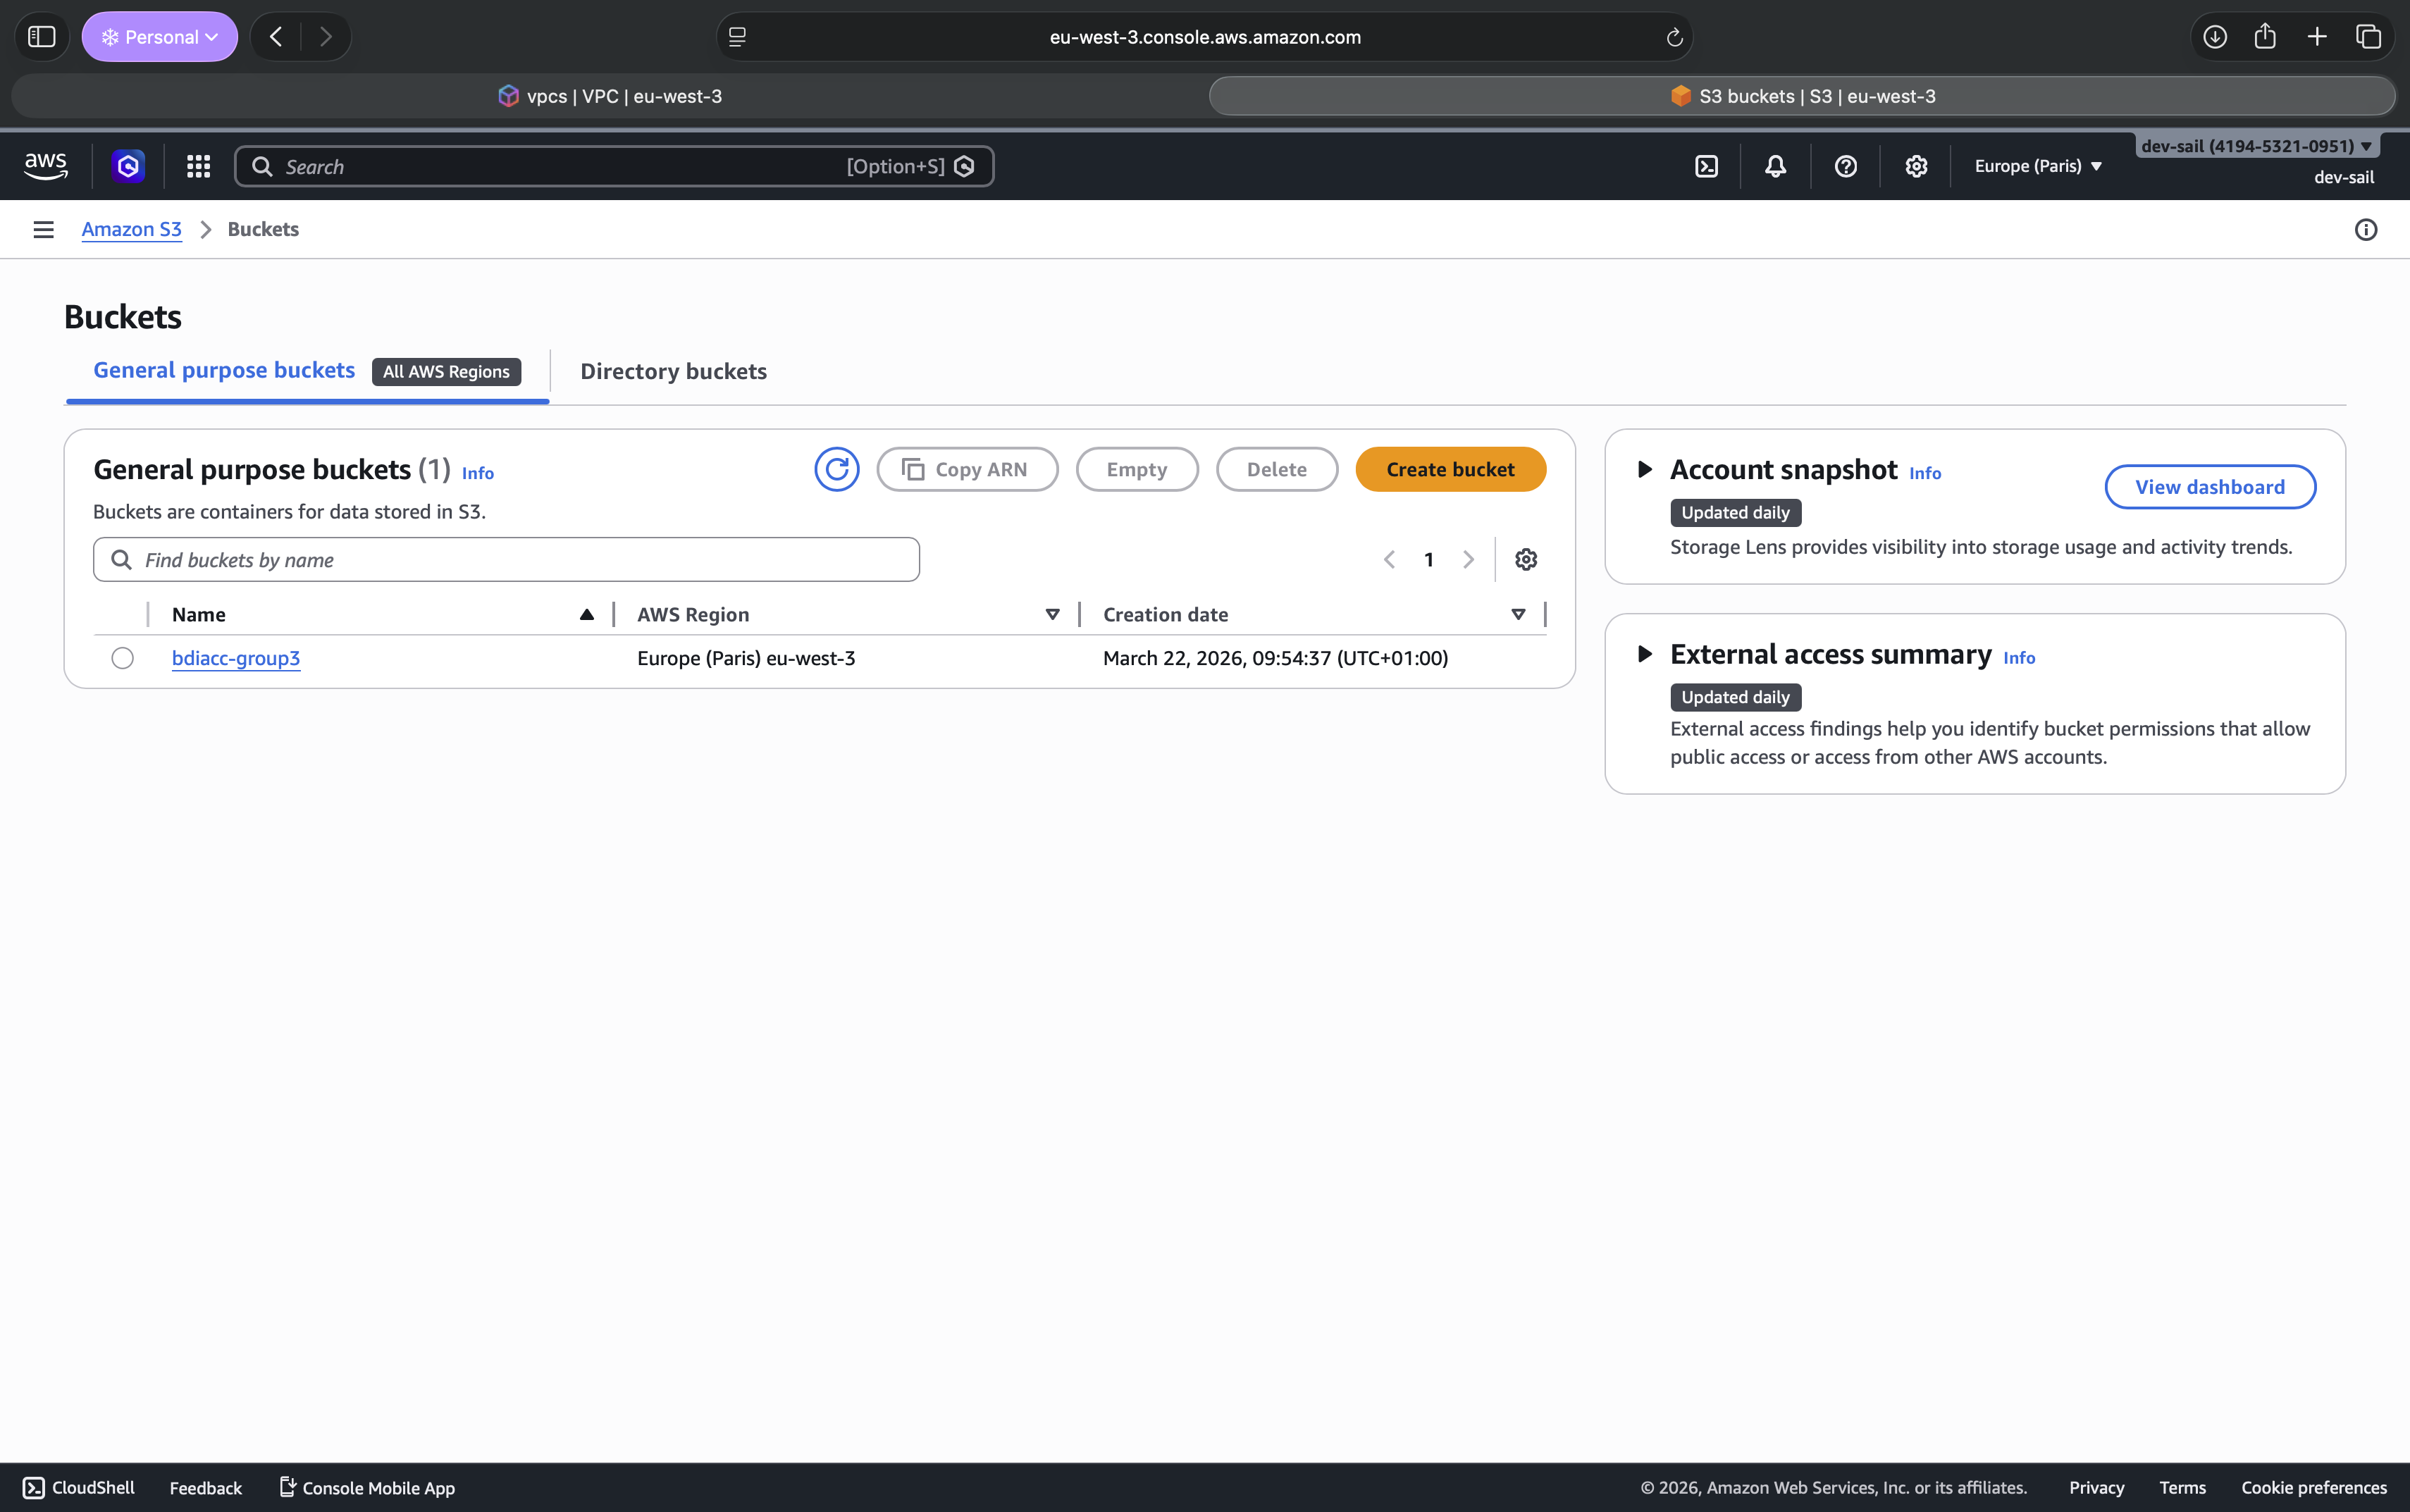
\includegraphics[width=0.75\textwidth]{figures/lab_4/s3_bucket_created.png}
\caption{S3 bucket created}
\end{figure}

\subsection{Upload 5 Objects with Different File Extensions}

We uploaded 5 different file types to the bucket to demonstrate how S3 handles various formats:

\begin{itemize}
    \item \texttt{requirement.txt} - 384.0 B
    \item \texttt{ch00.pdf} - 142.7 KB
    \item \texttt{main.py} - 2.4 KB
    \item \texttt{setup.md} - 5.6 KB
    \item \texttt{favicon.ico} - 15.0 KB
\end{itemize}

\begin{figure}[H]
\centering
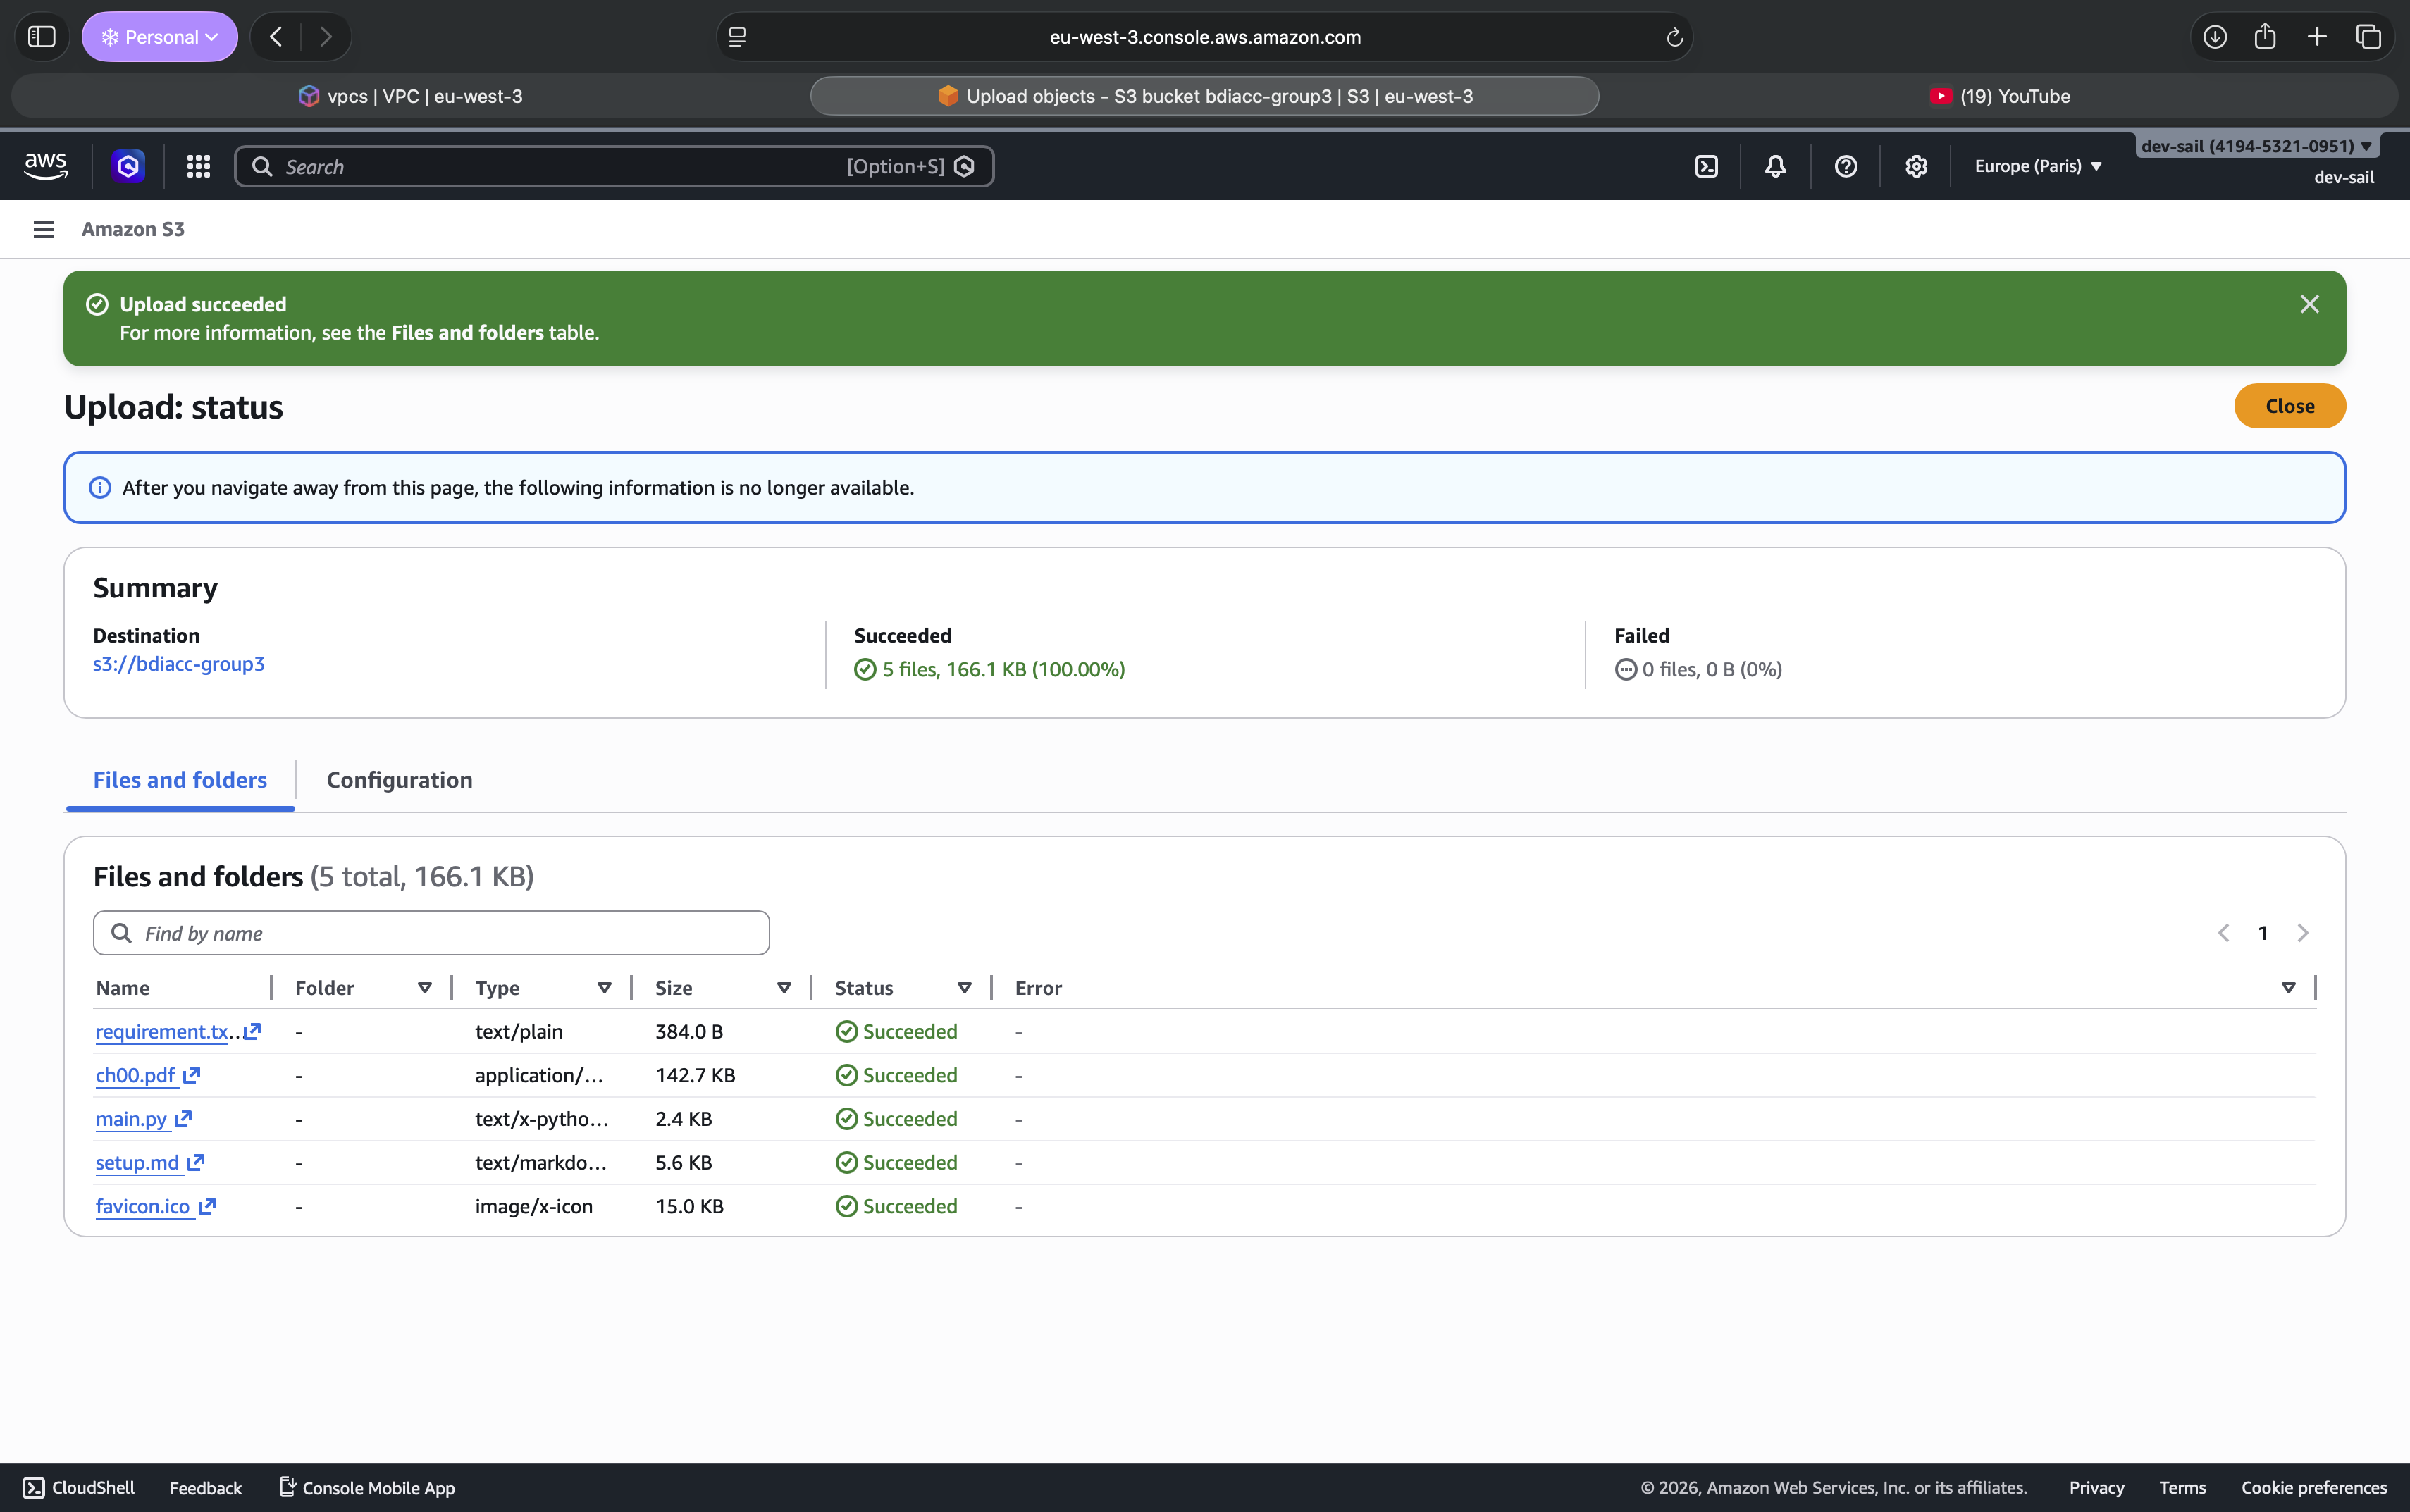
\includegraphics[width=0.75\textwidth]{figures/lab_4/upload_5_different_types_of_files.png}
\caption{Objects uploaded to S3 bucket}
\end{figure}

All files uploaded correctly using the drag-and-drop interface.
\vspace{14cm}
%% ============ SECTION 2: S3 Static Website Hosting ============ %%
\section{S3 Static Website Hosting}

\subsection{Enable Static Website Hosting}

We enabled static website hosting on the bucket. This allows the bucket to serve HTML content directly over HTTP.

\textbf{Configuration:}
\begin{itemize}
    \item \textbf{Index document:} index.html
    \item \textbf{Error document:} error.html
\end{itemize}

\begin{figure}[H]
\centering
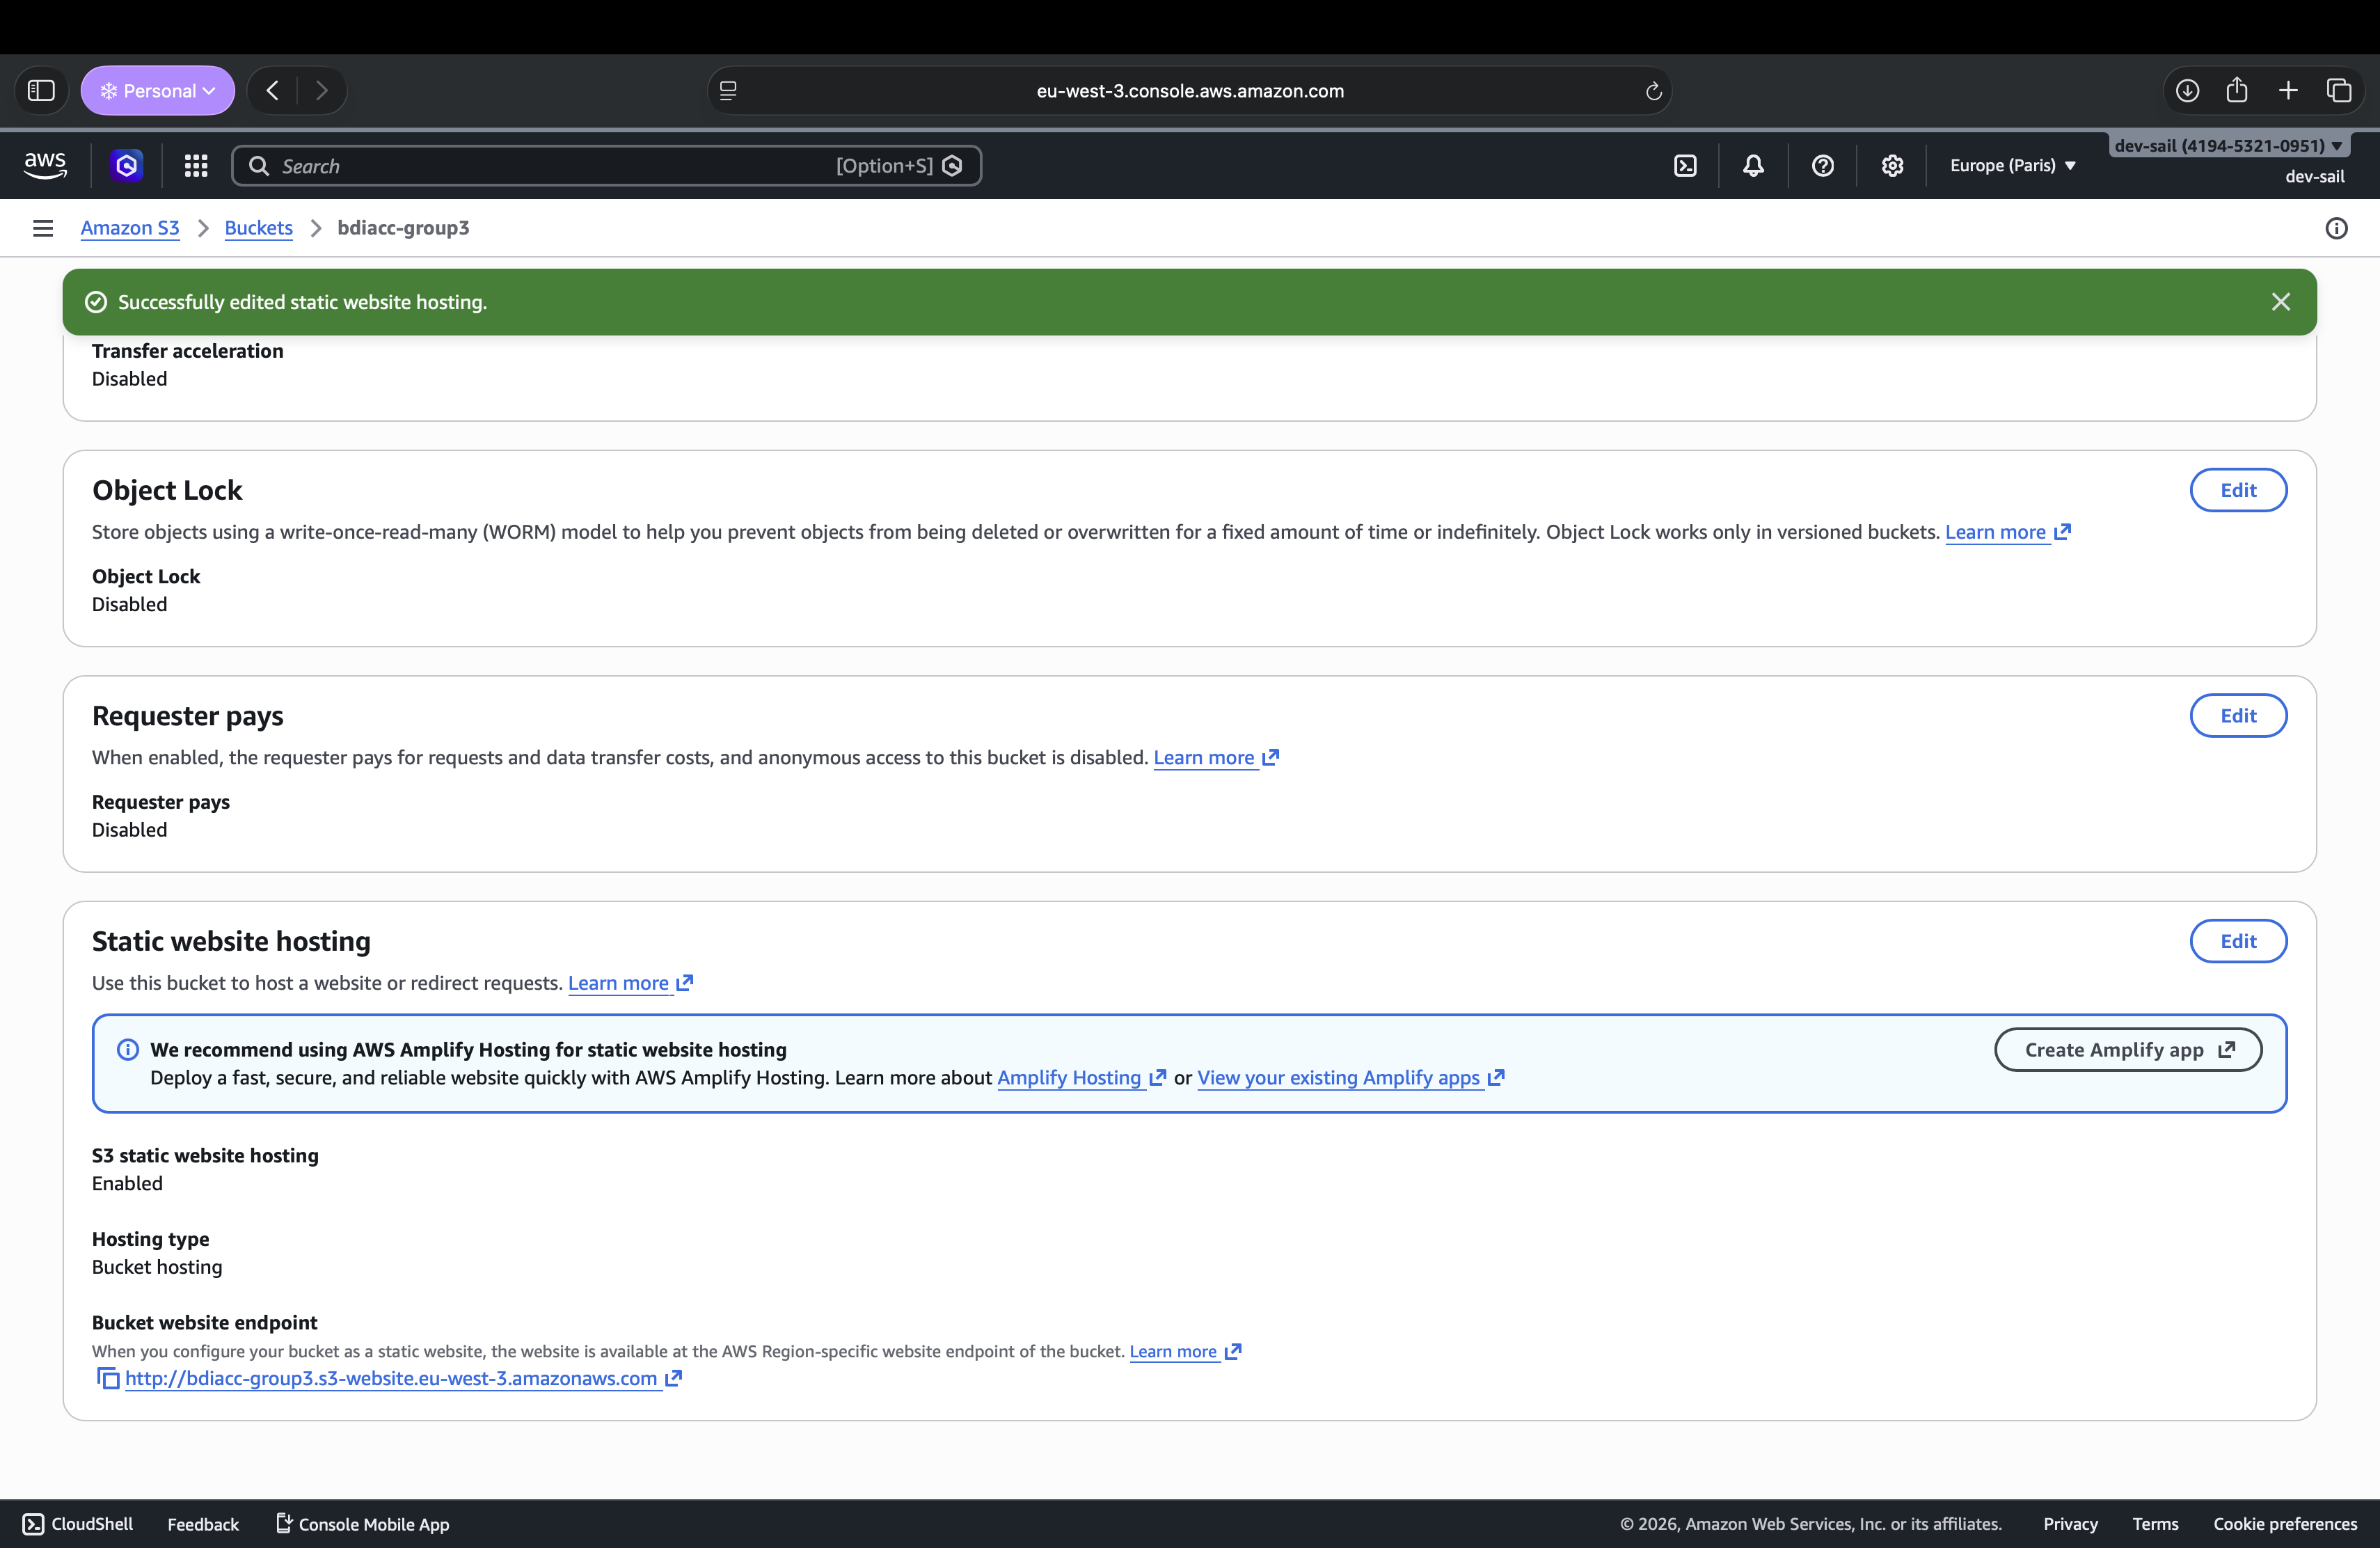
\includegraphics[width=0.75\textwidth]{figures/lab_4/static_website_hosting_configured.png}
\caption{Static website hosting enabled}
\end{figure}

The endpoint provided by AWS is:
\begin{center}
\texttt{http://bdiacc-group3.s3-website.eu-west-3.amazonaws.com}
\end{center}

\subsection{Upload index.html and error.html Files}

We uploaded HTML files to support the website. The index.html page shows group information:

\begin{itemize}
    \item S3 Bucket: bdiacc-group3
    \item Group 3
    \item Big Data Infrastructure and Cloud Computing
    \item MSc Computer Science, Software Engineering
    \item Team: Jordy Meye, Huizhe Su, Arihant Jain, Nizar
\end{itemize}

The error.html displays a 404 page with a "Go back" link for users who request missing pages.

\subsection{Configure Bucket Policy for Public Access}

When we first tried to access the website, we got a 403 Forbidden error because the bucket was set to block all public access.

\begin{figure}[H]
\centering
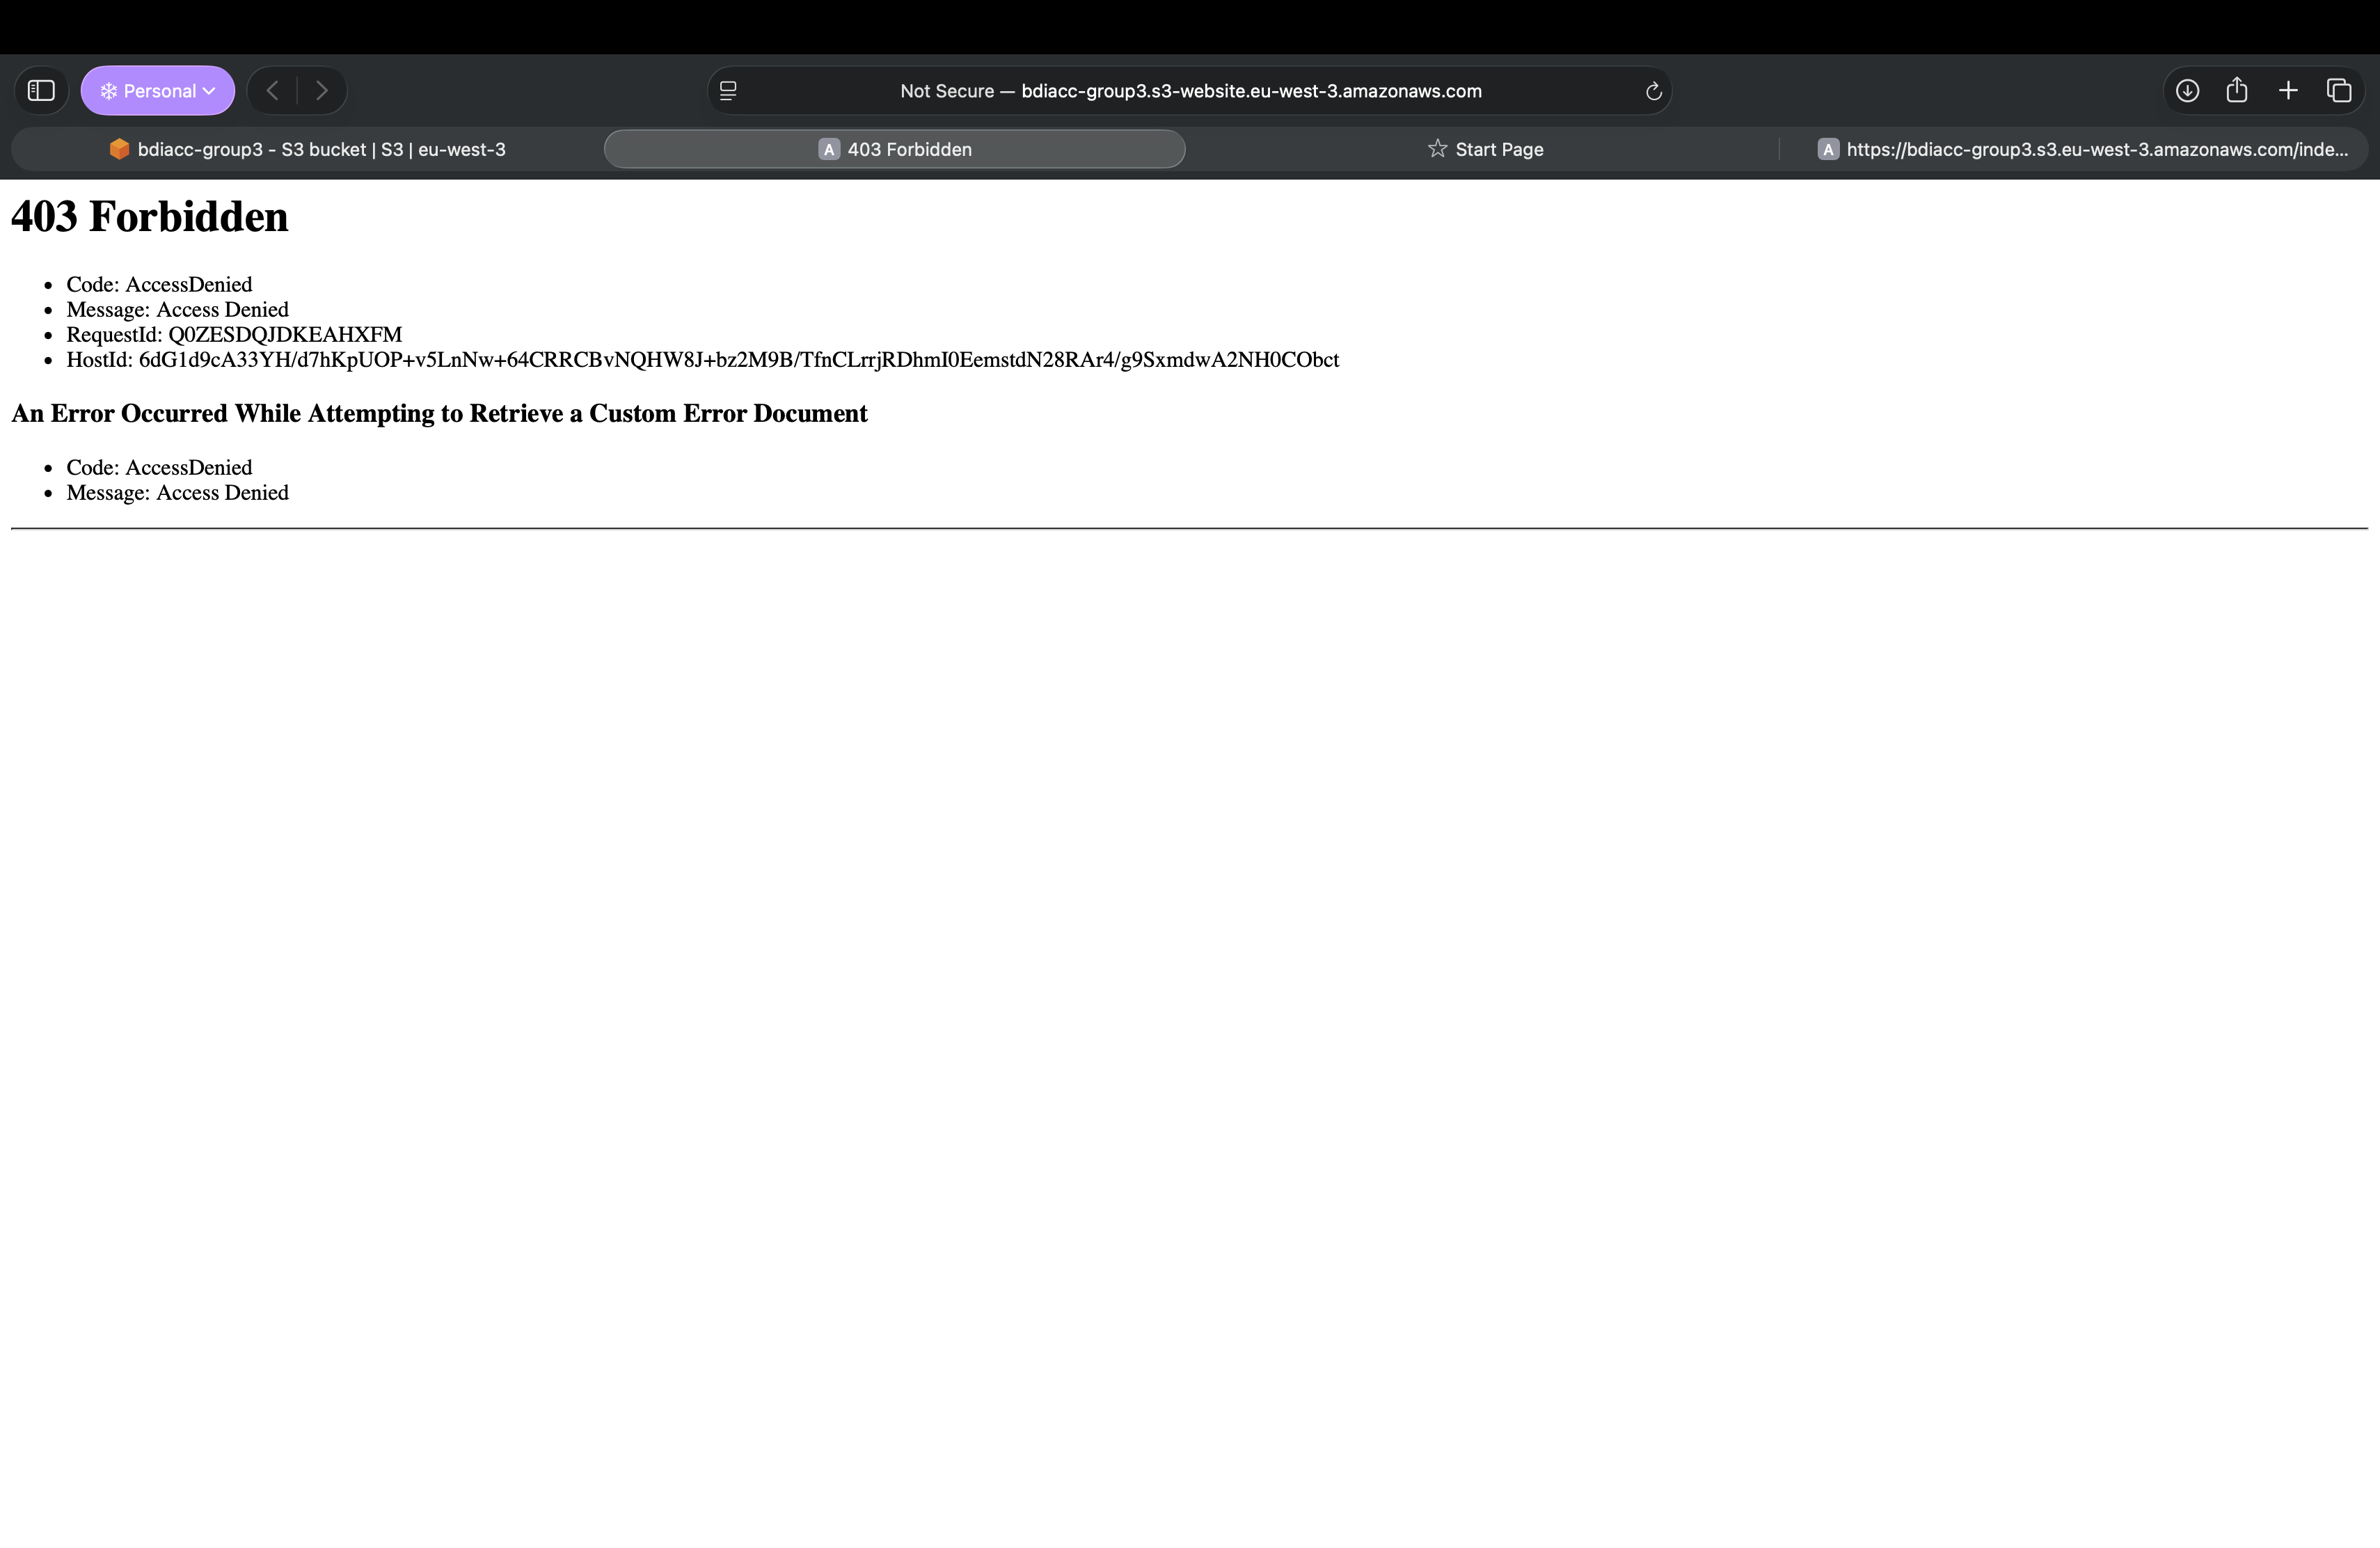
\includegraphics[width=0.75\textwidth]{figures/lab_4/access_error_before_bucket_policy.png}
\caption{403 error before bucket policy}
\end{figure}

\vspace{-0.3cm}

We added a bucket policy to allow public read access:

\begin{lstlisting}
{
    "Version": "2012-10-17",
    "Statement": [
        {
            "Sid": "PublicReadGetObject",
            "Effect": "Allow",
            "Principal": "*",
            "Action": "s3:GetObject",
            "Resource": "arn:aws:s3:::bdiacc-group3/*"
        }
    ]
}
\end{lstlisting}

\subsection{View HTML Files}

After applying the policy, both files became accessible through the S3 website endpoint.

\begin{figure}[H]
\centering
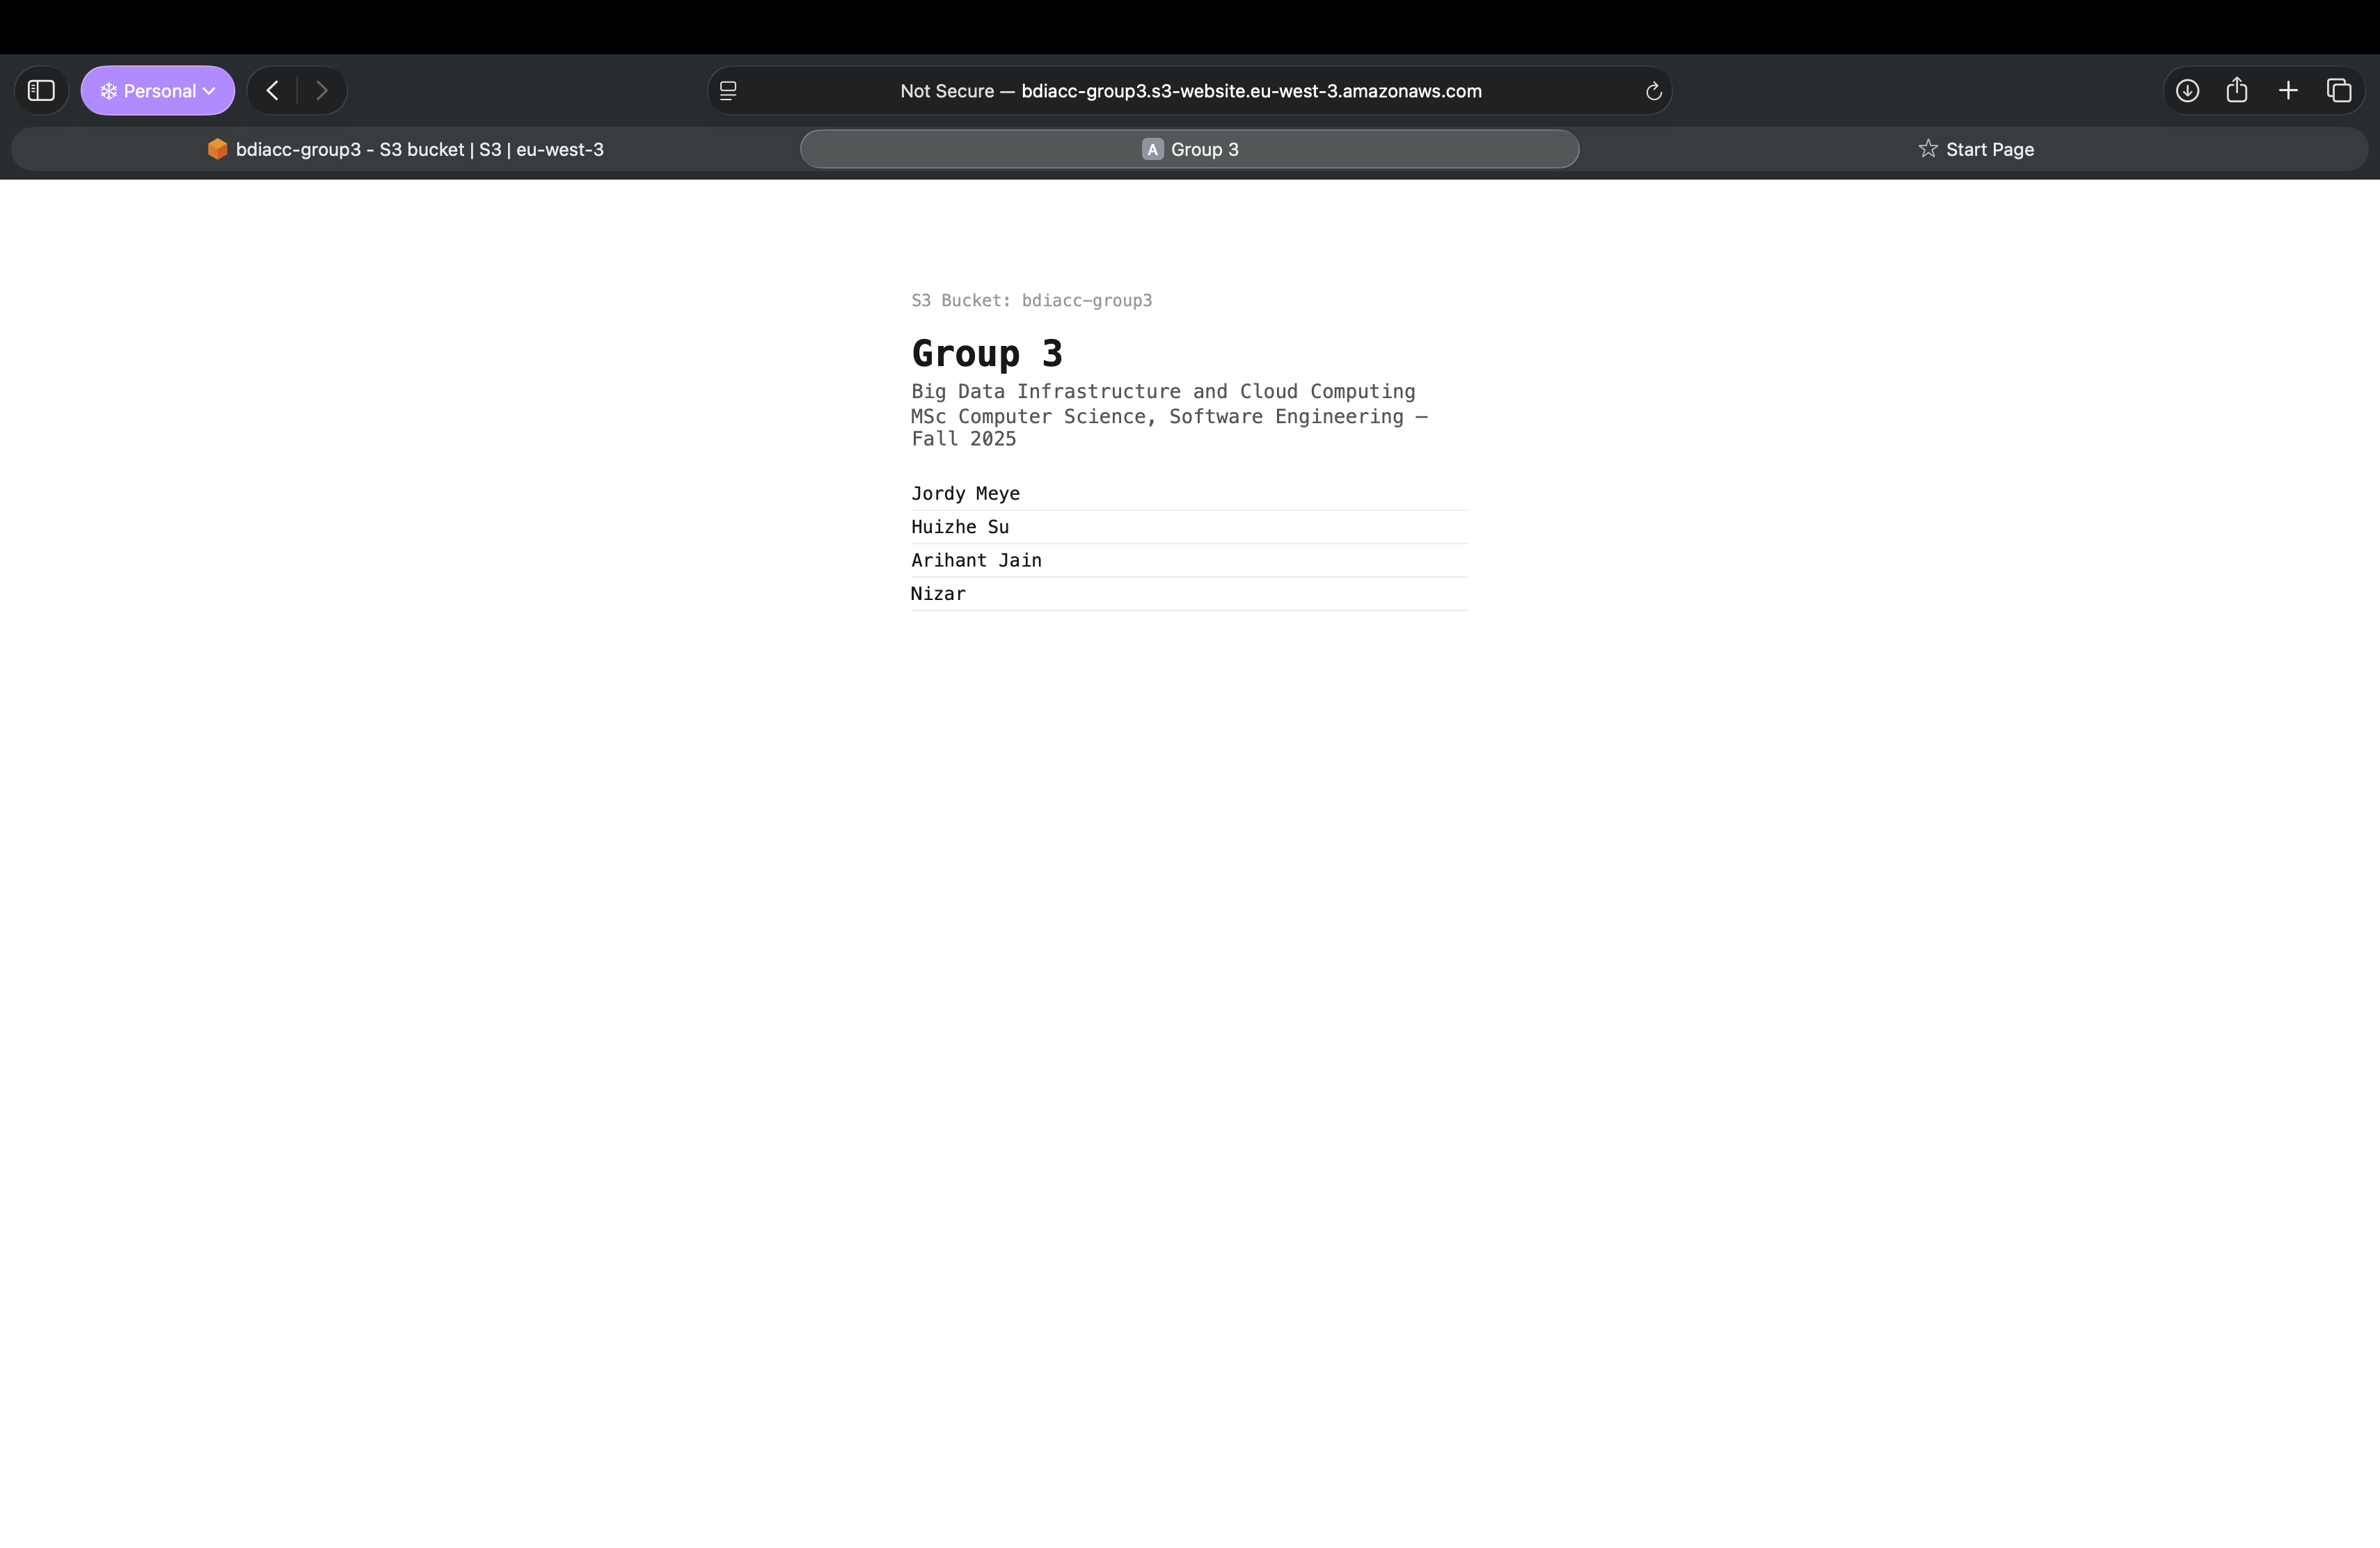
\includegraphics[width=0.75\textwidth]{figures/lab_4/index_html.png}
\caption{index.html}
\end{figure}

\begin{figure}[H]
\centering
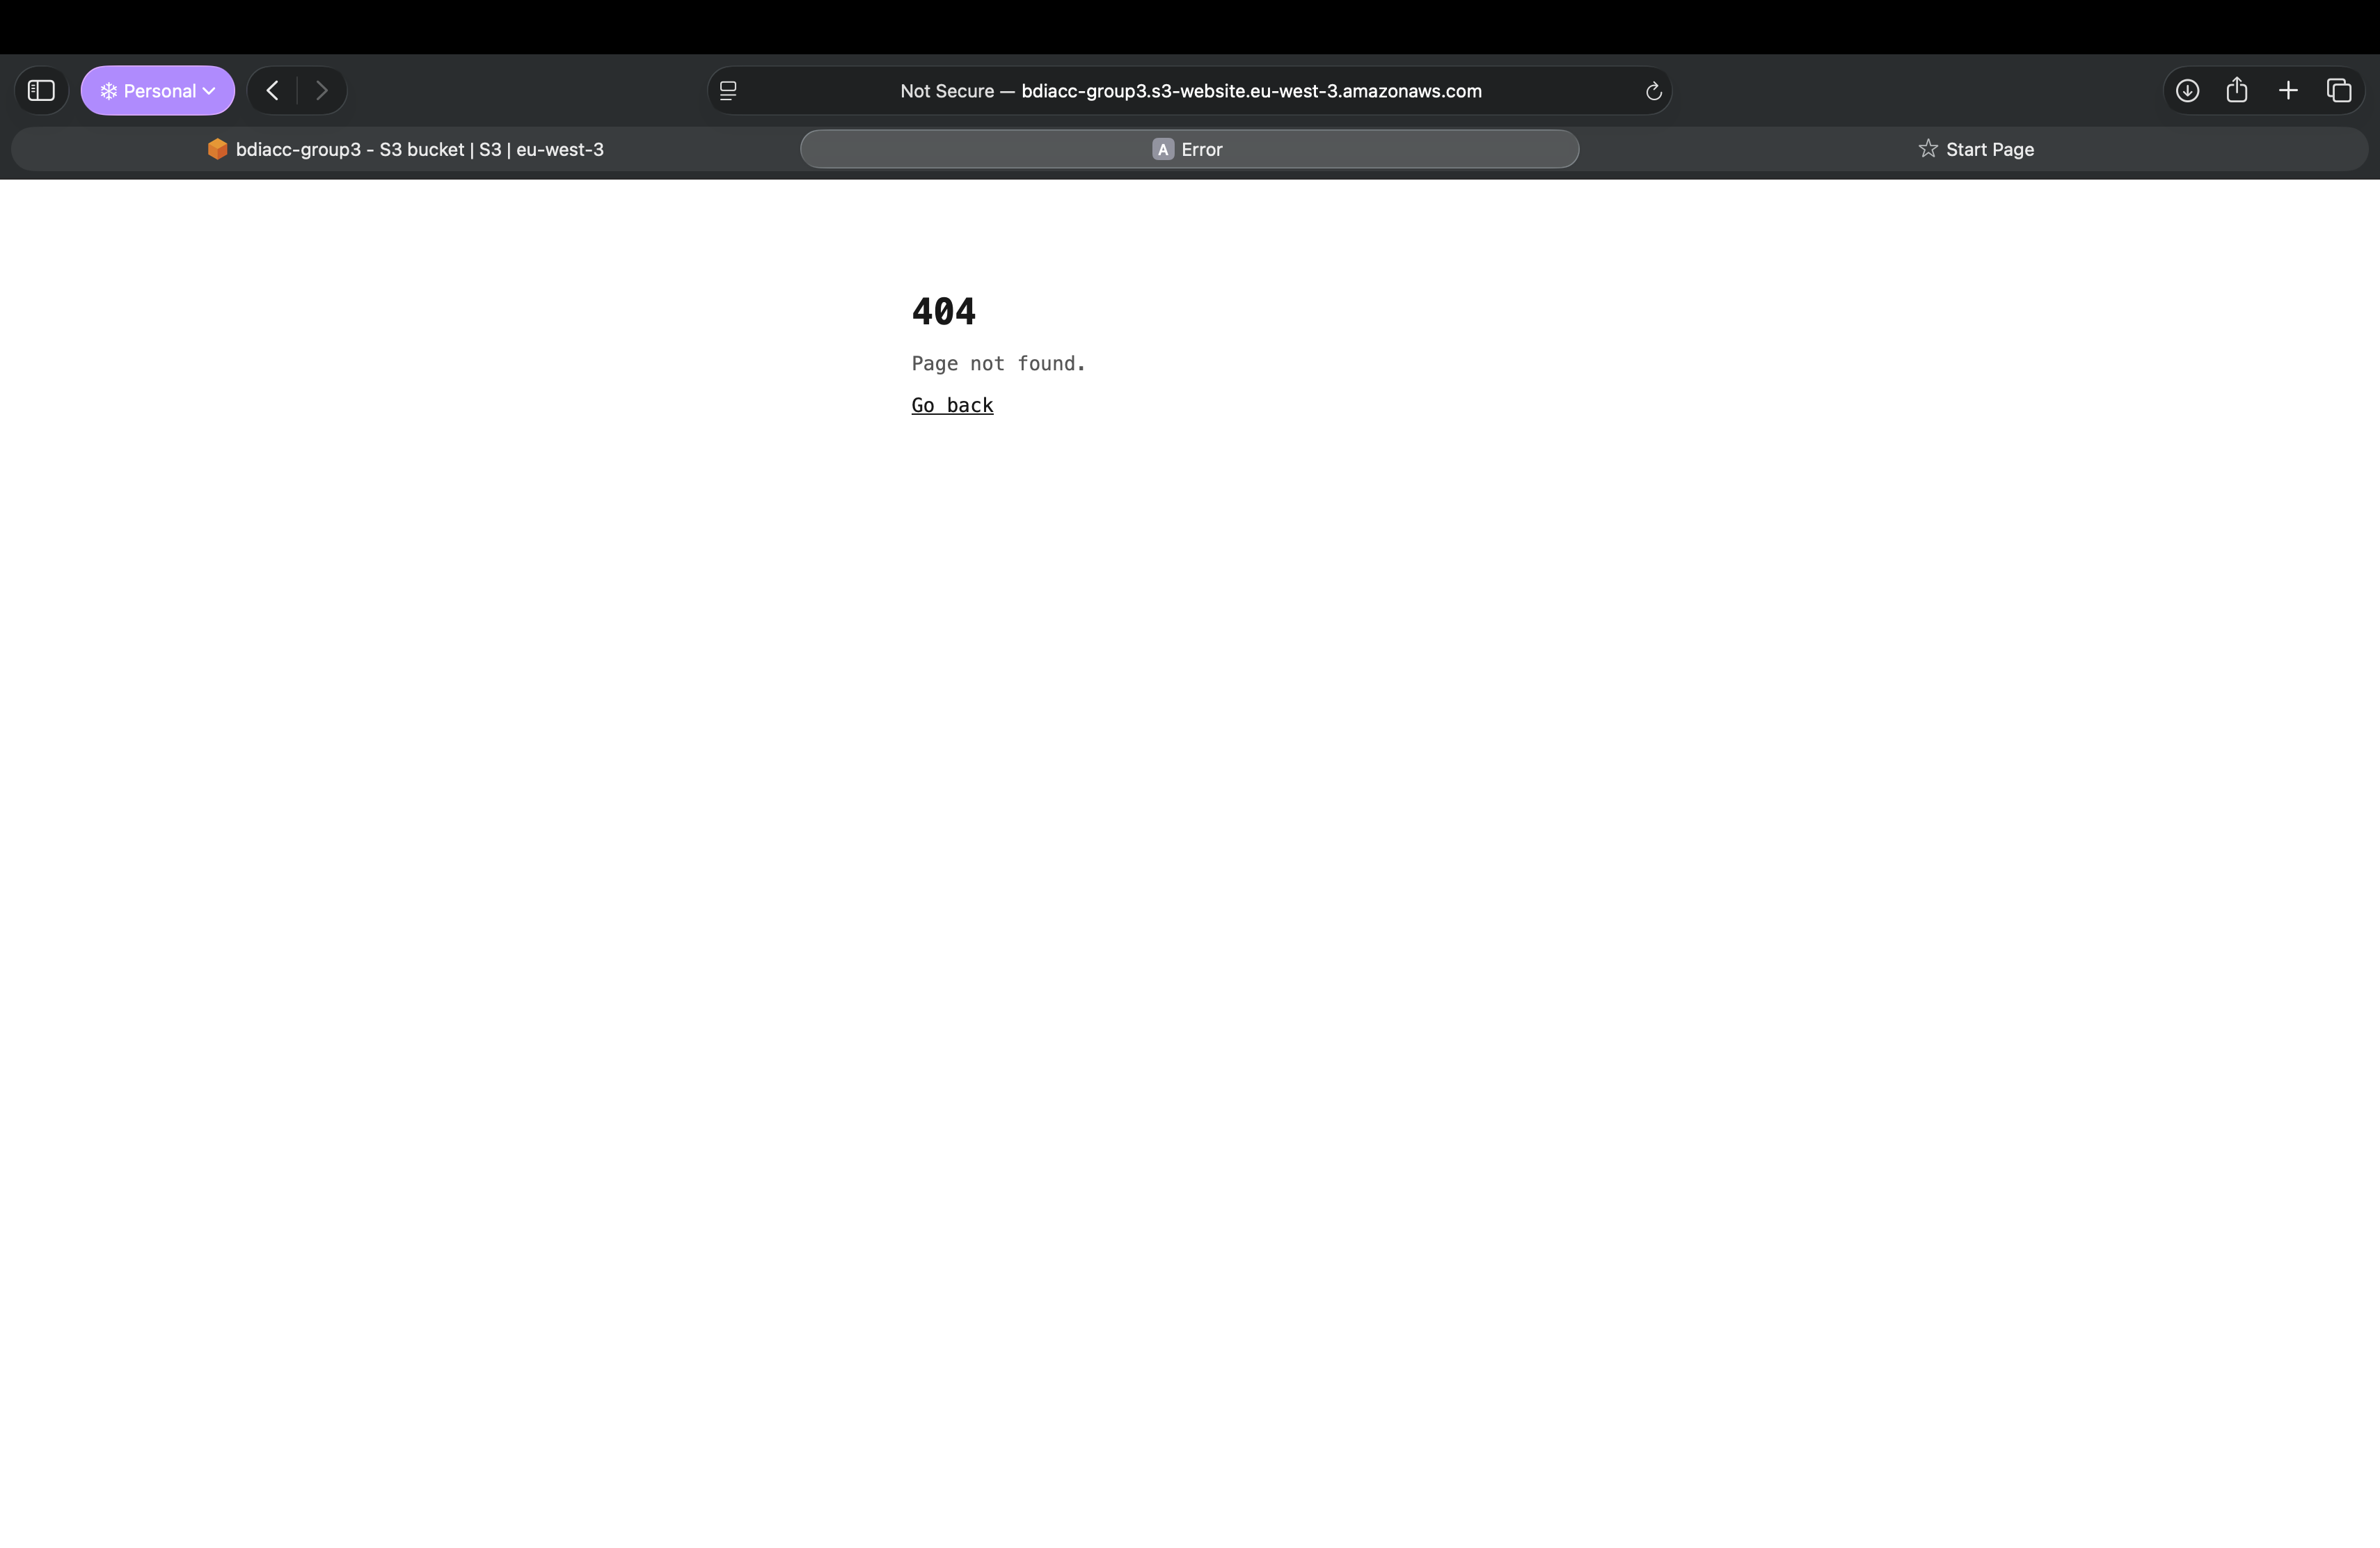
\includegraphics[width=0.75\textwidth]{figures/lab_4/error_html.png}
\caption{error.html}
\end{figure}

\subsection{Add Lifecycle Rules}

We configured a lifecycle rule named "StorageClassChange" with the following settings:

\begin{itemize}
    \item Day 60: Move objects to Standard-IA storage class
    \item Day 200: Delete objects
    \item For noncurrent versions: Keep 2 newest versions, move others to Standard-IA at day 30
\end{itemize}

\begin{figure}[H]
\centering
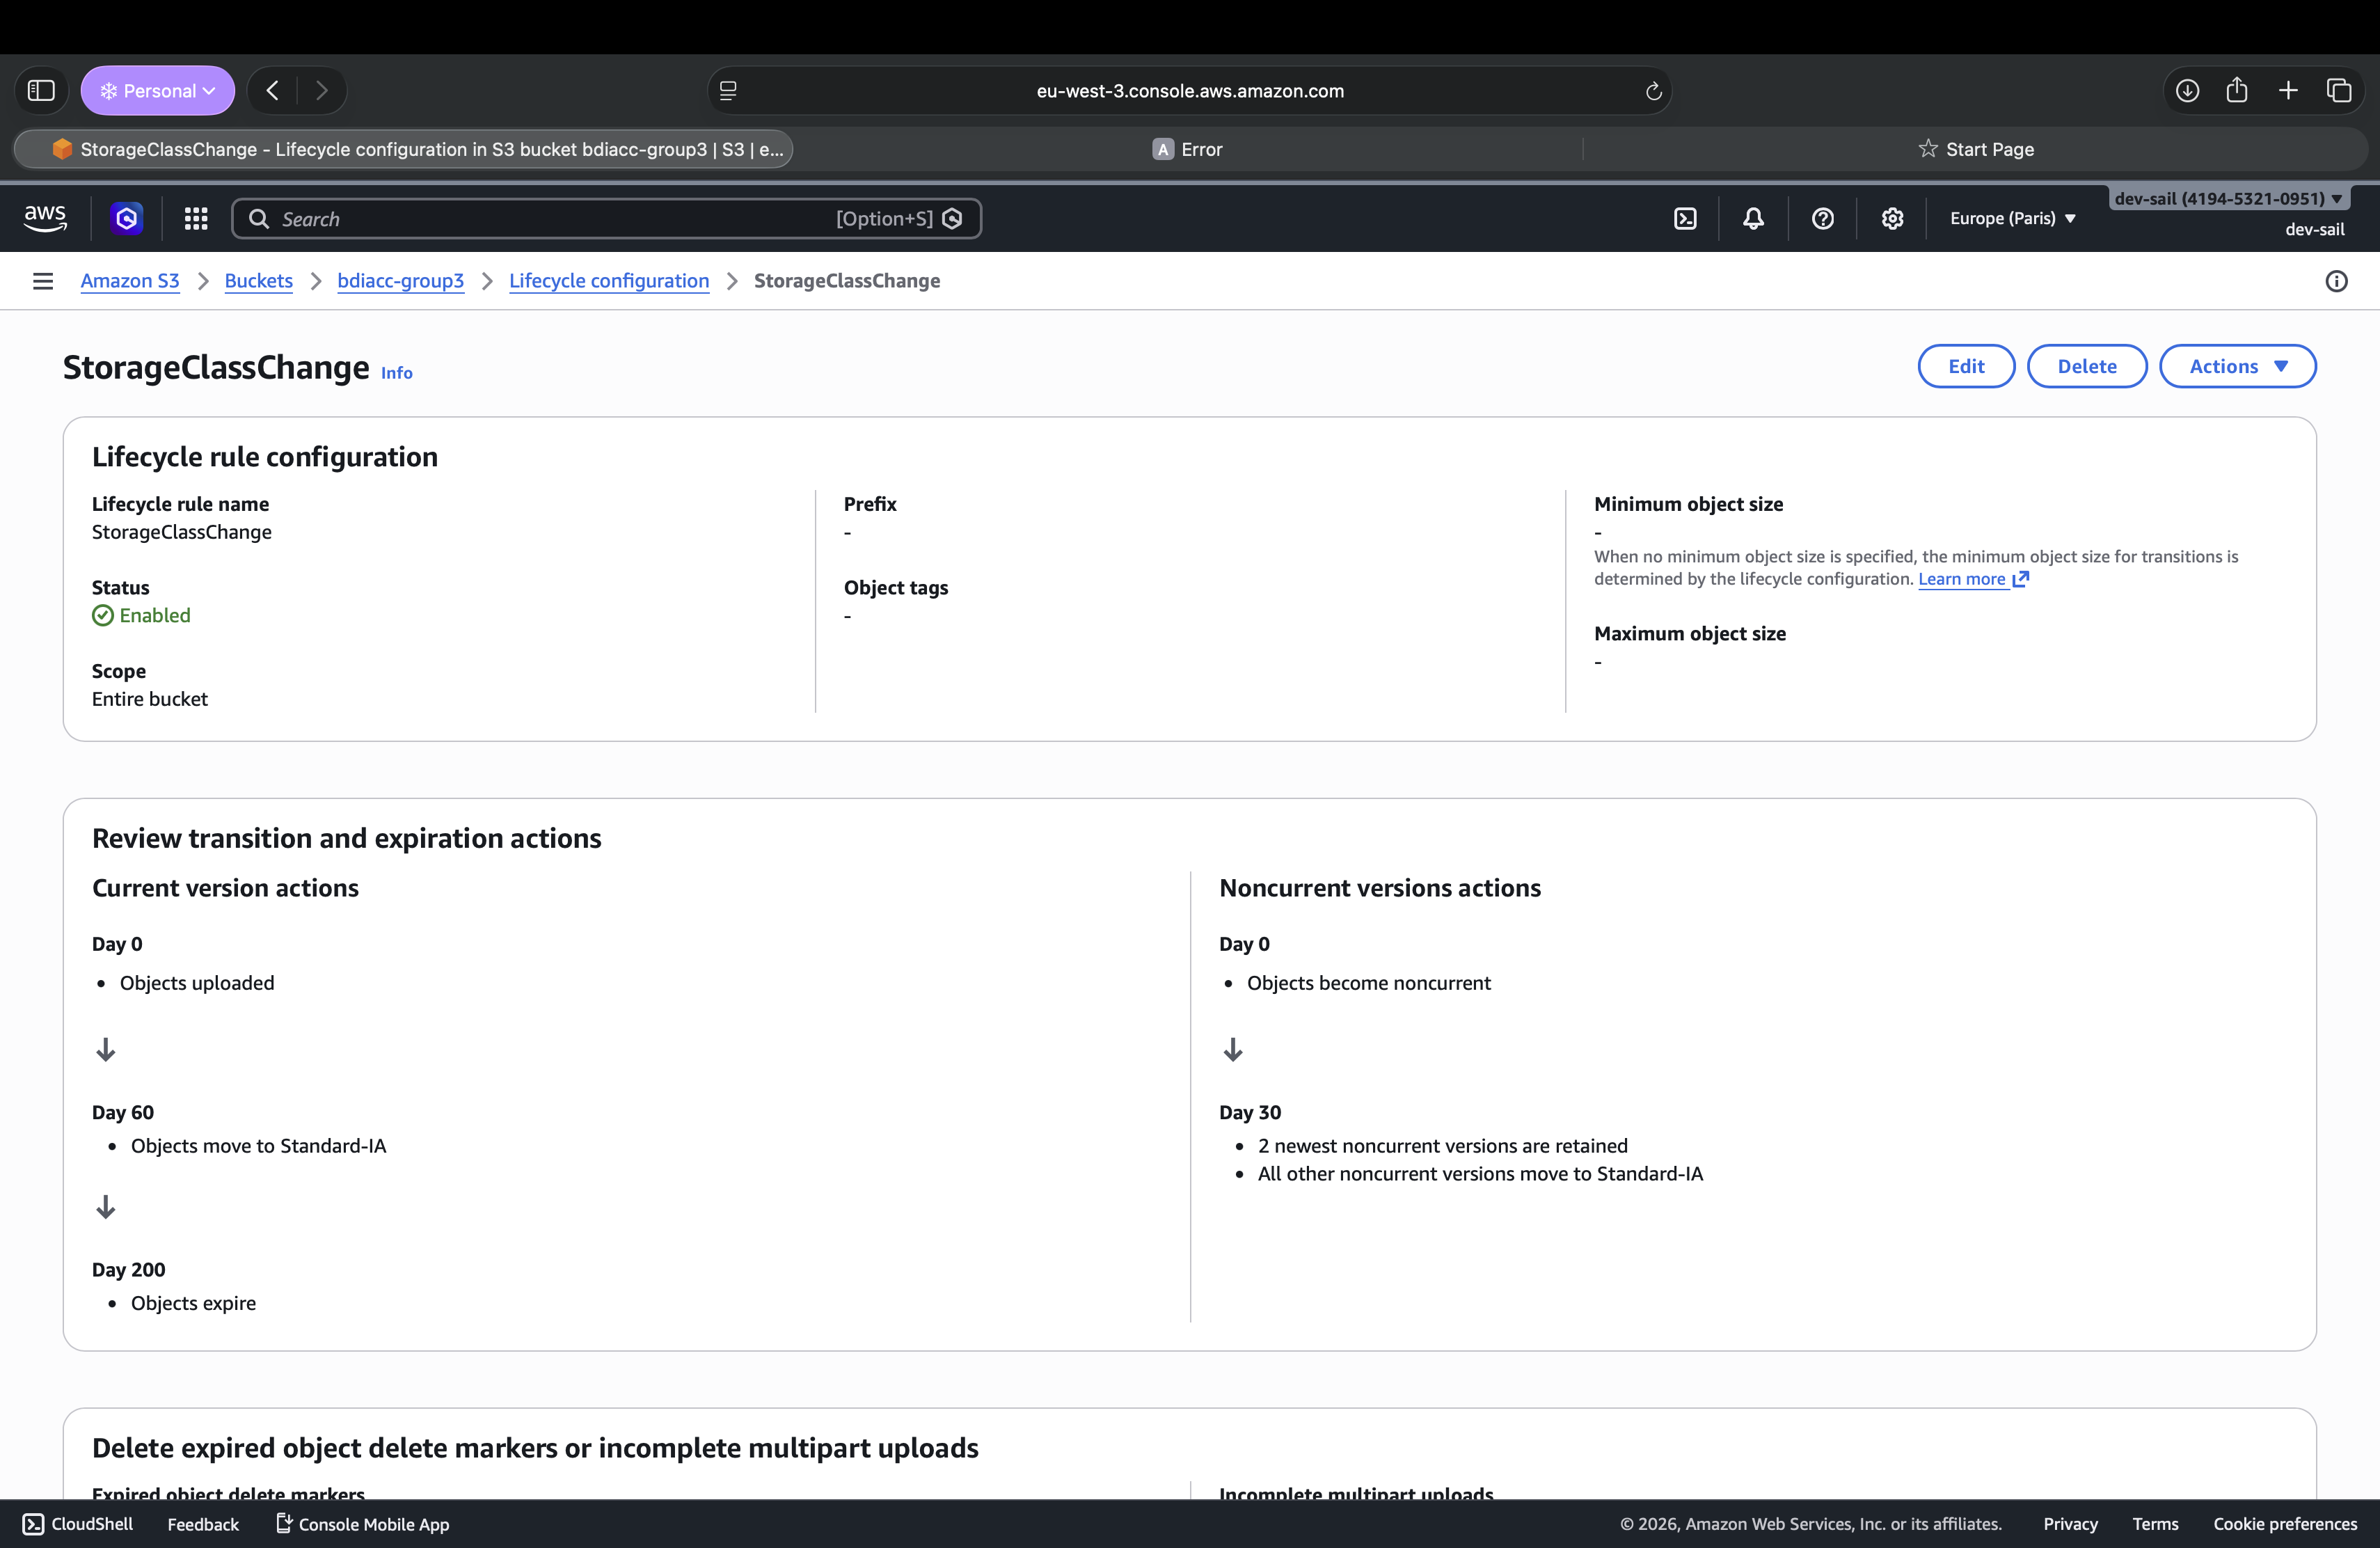
\includegraphics[width=0.75\textwidth]{figures/lab_4/lifecycle_rule_configuration.png}
\caption{Lifecycle rule configuration}
\end{figure}

This reduces storage costs by automatically moving old objects to cheaper storage or deleting them.
\vspace{11cm}
%% ============ SECTION 3: S3 Bucket Versioning ============ %%
\section{S3 Bucket Versioning}

\subsection{Enable Versioning for the Bucket}

We enabled versioning on the bucket so that previous versions of files are kept when they are updated.

\begin{figure}[H]
\centering
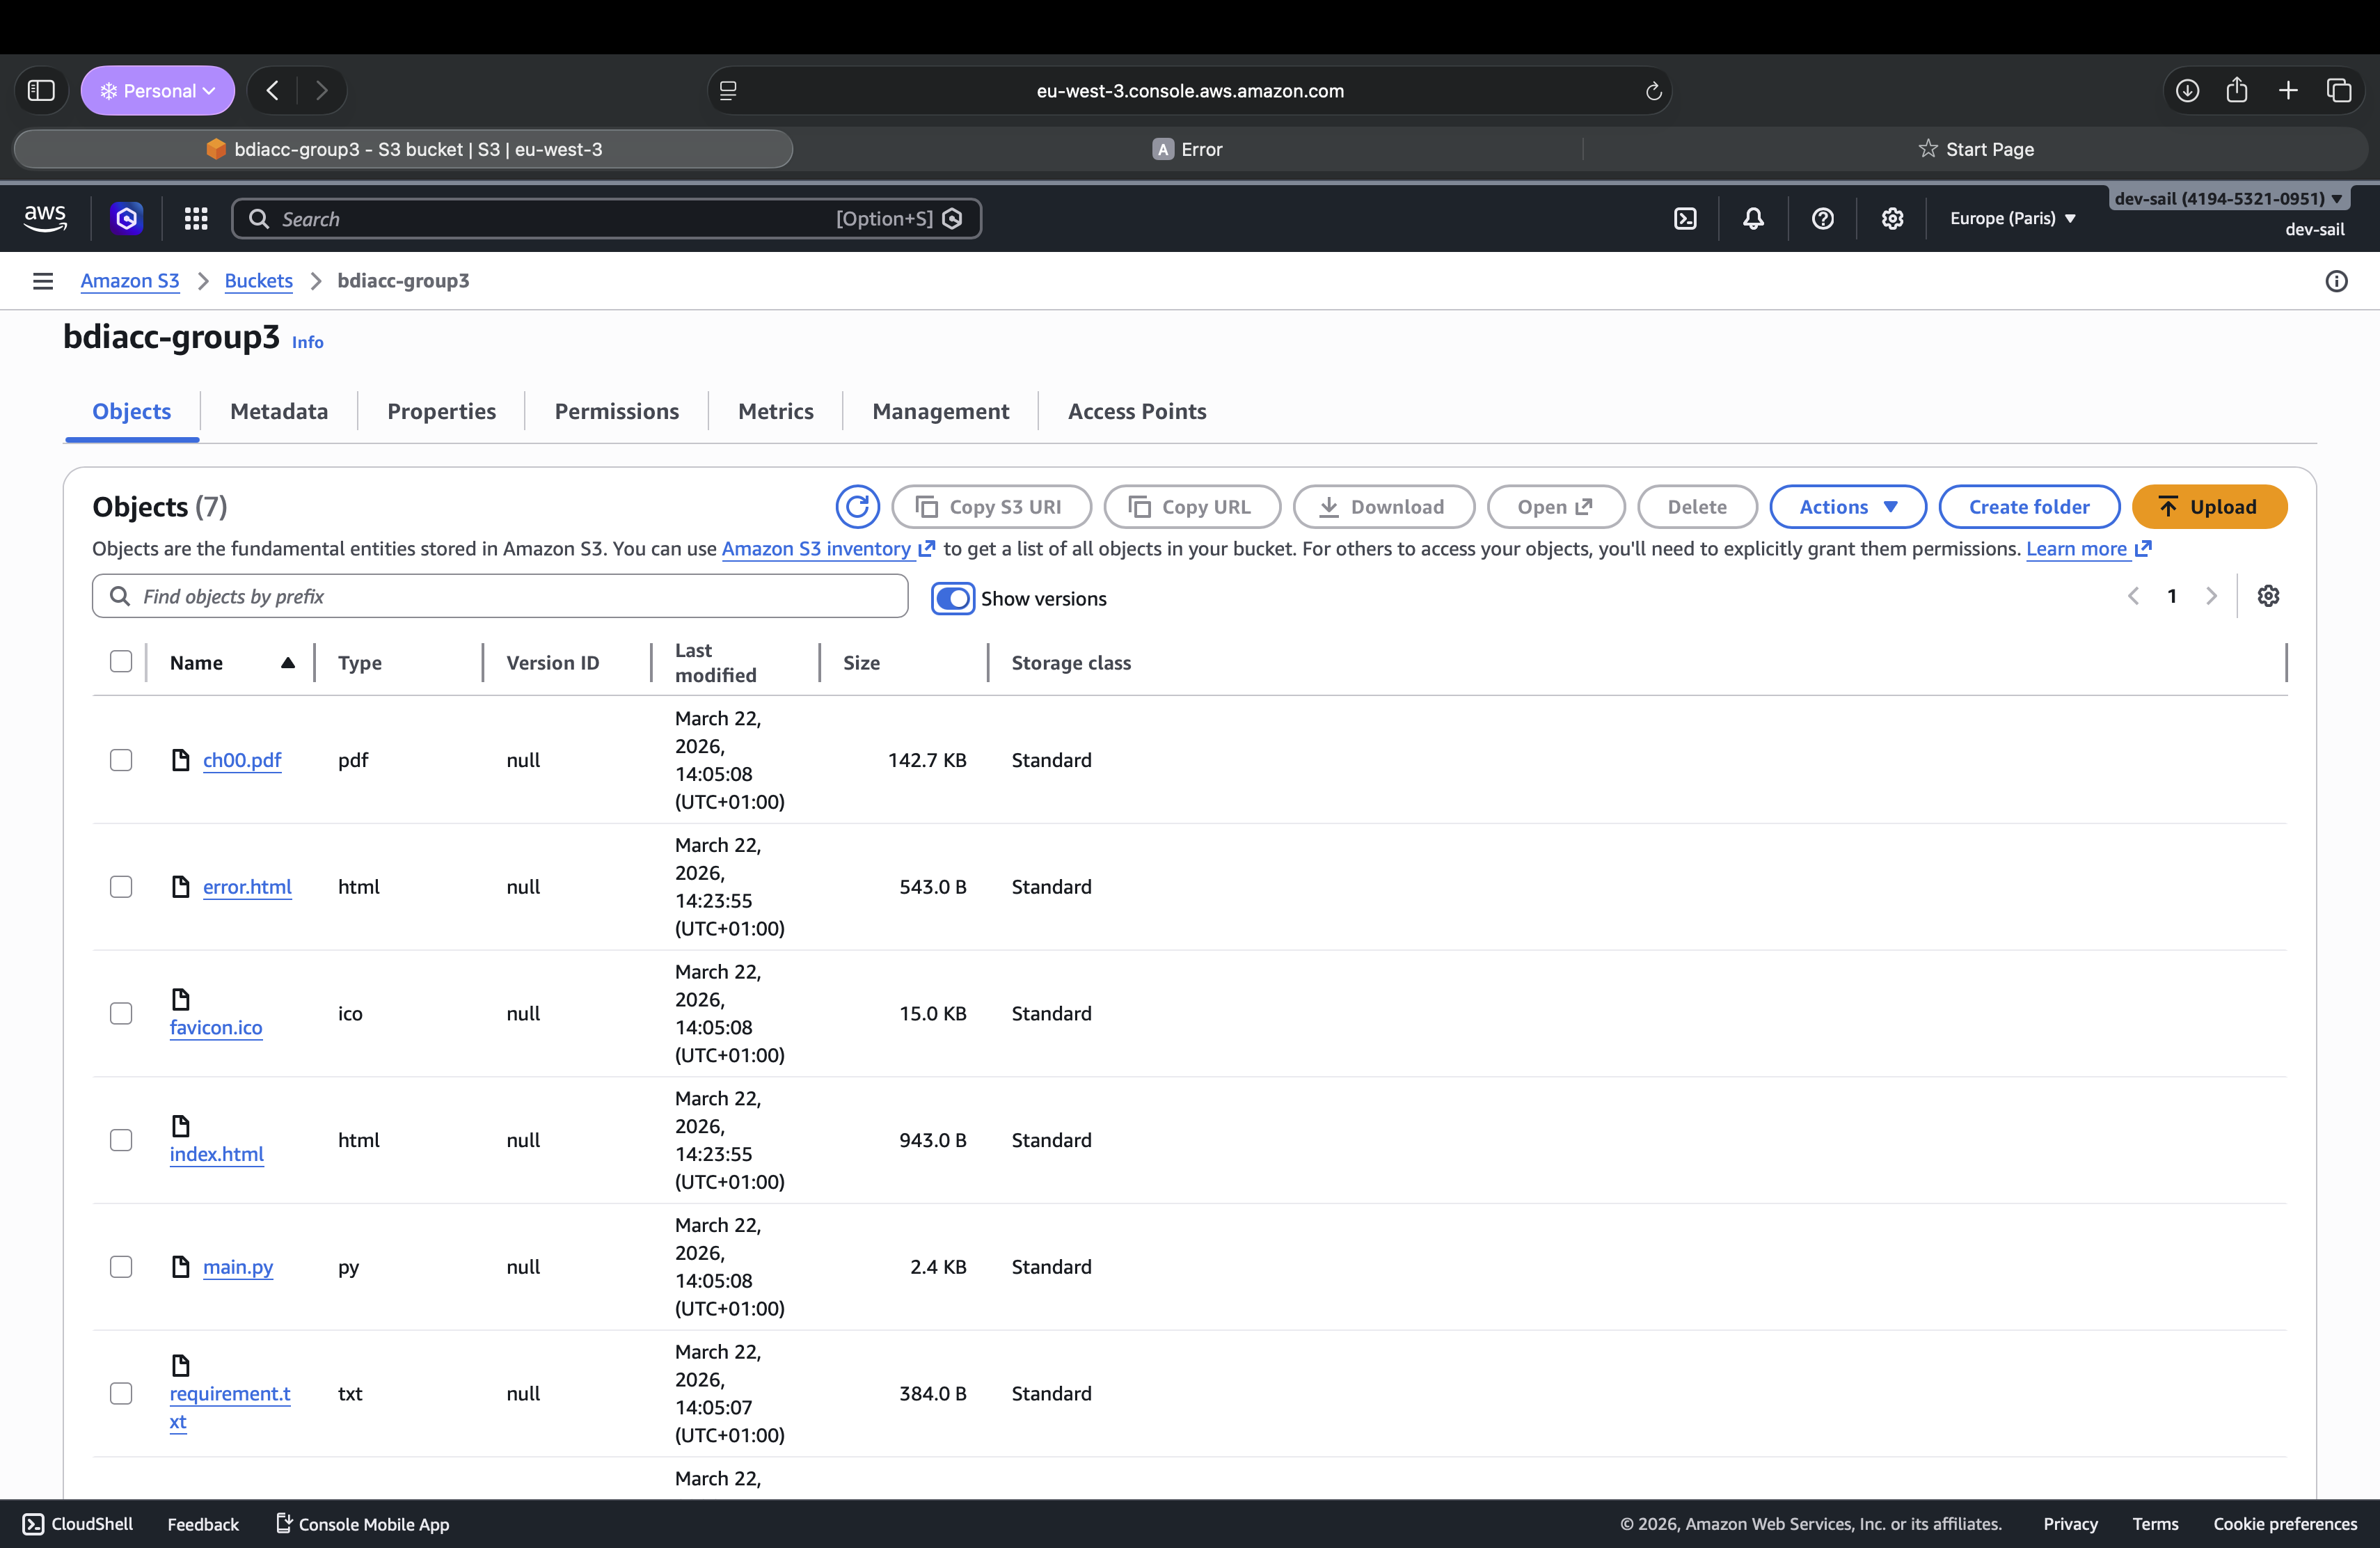
\includegraphics[width=0.75\textwidth]{figures/lab_4/object_versioning_on.png}
\caption{Versioning enabled}
\end{figure}

Once enabled, every object gets a unique version ID. Old versions can be restored if needed.

\subsection{Re-upload Files and Verify Versioning}

We uploaded new versions of index.html and error.html to test how versioning works. S3 keeps both the old and new versions.

\textbf{Original versions:}

\begin{figure}[H]
\centering
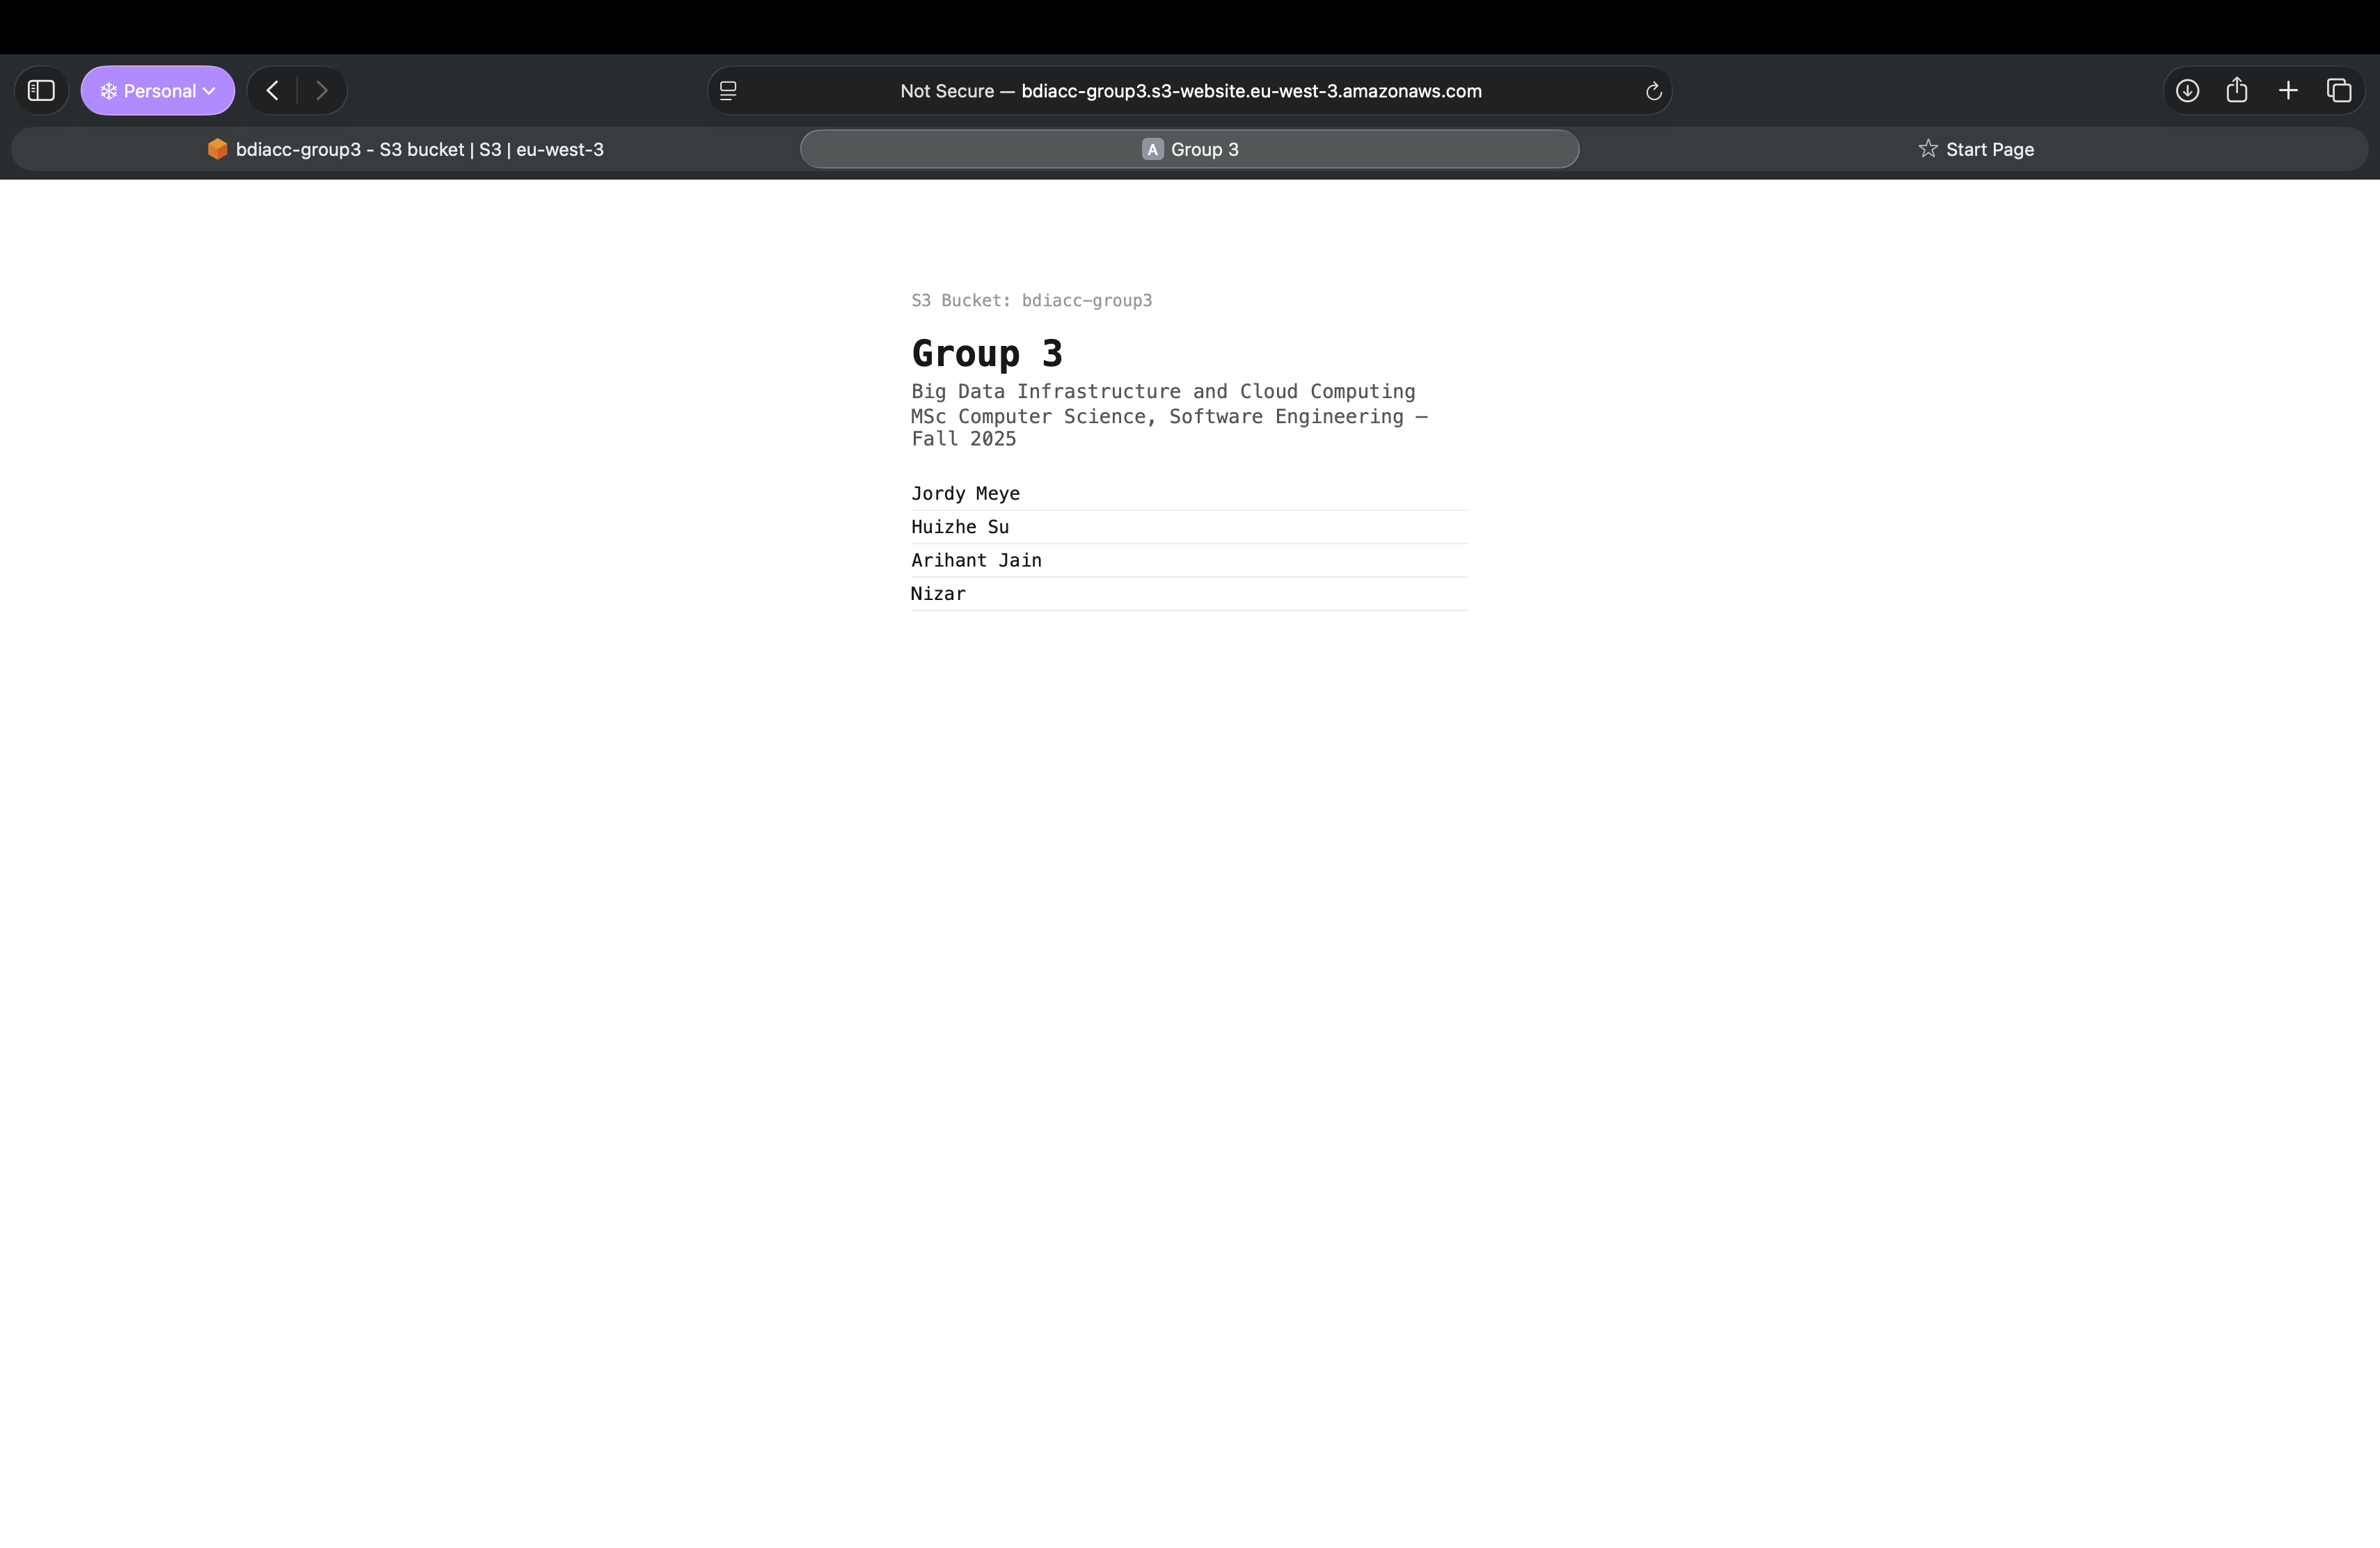
\includegraphics[width=0.75\textwidth]{figures/lab_4/index_html.png}
\caption{Original index.html}
\end{figure}

\begin{figure}[H]
\centering
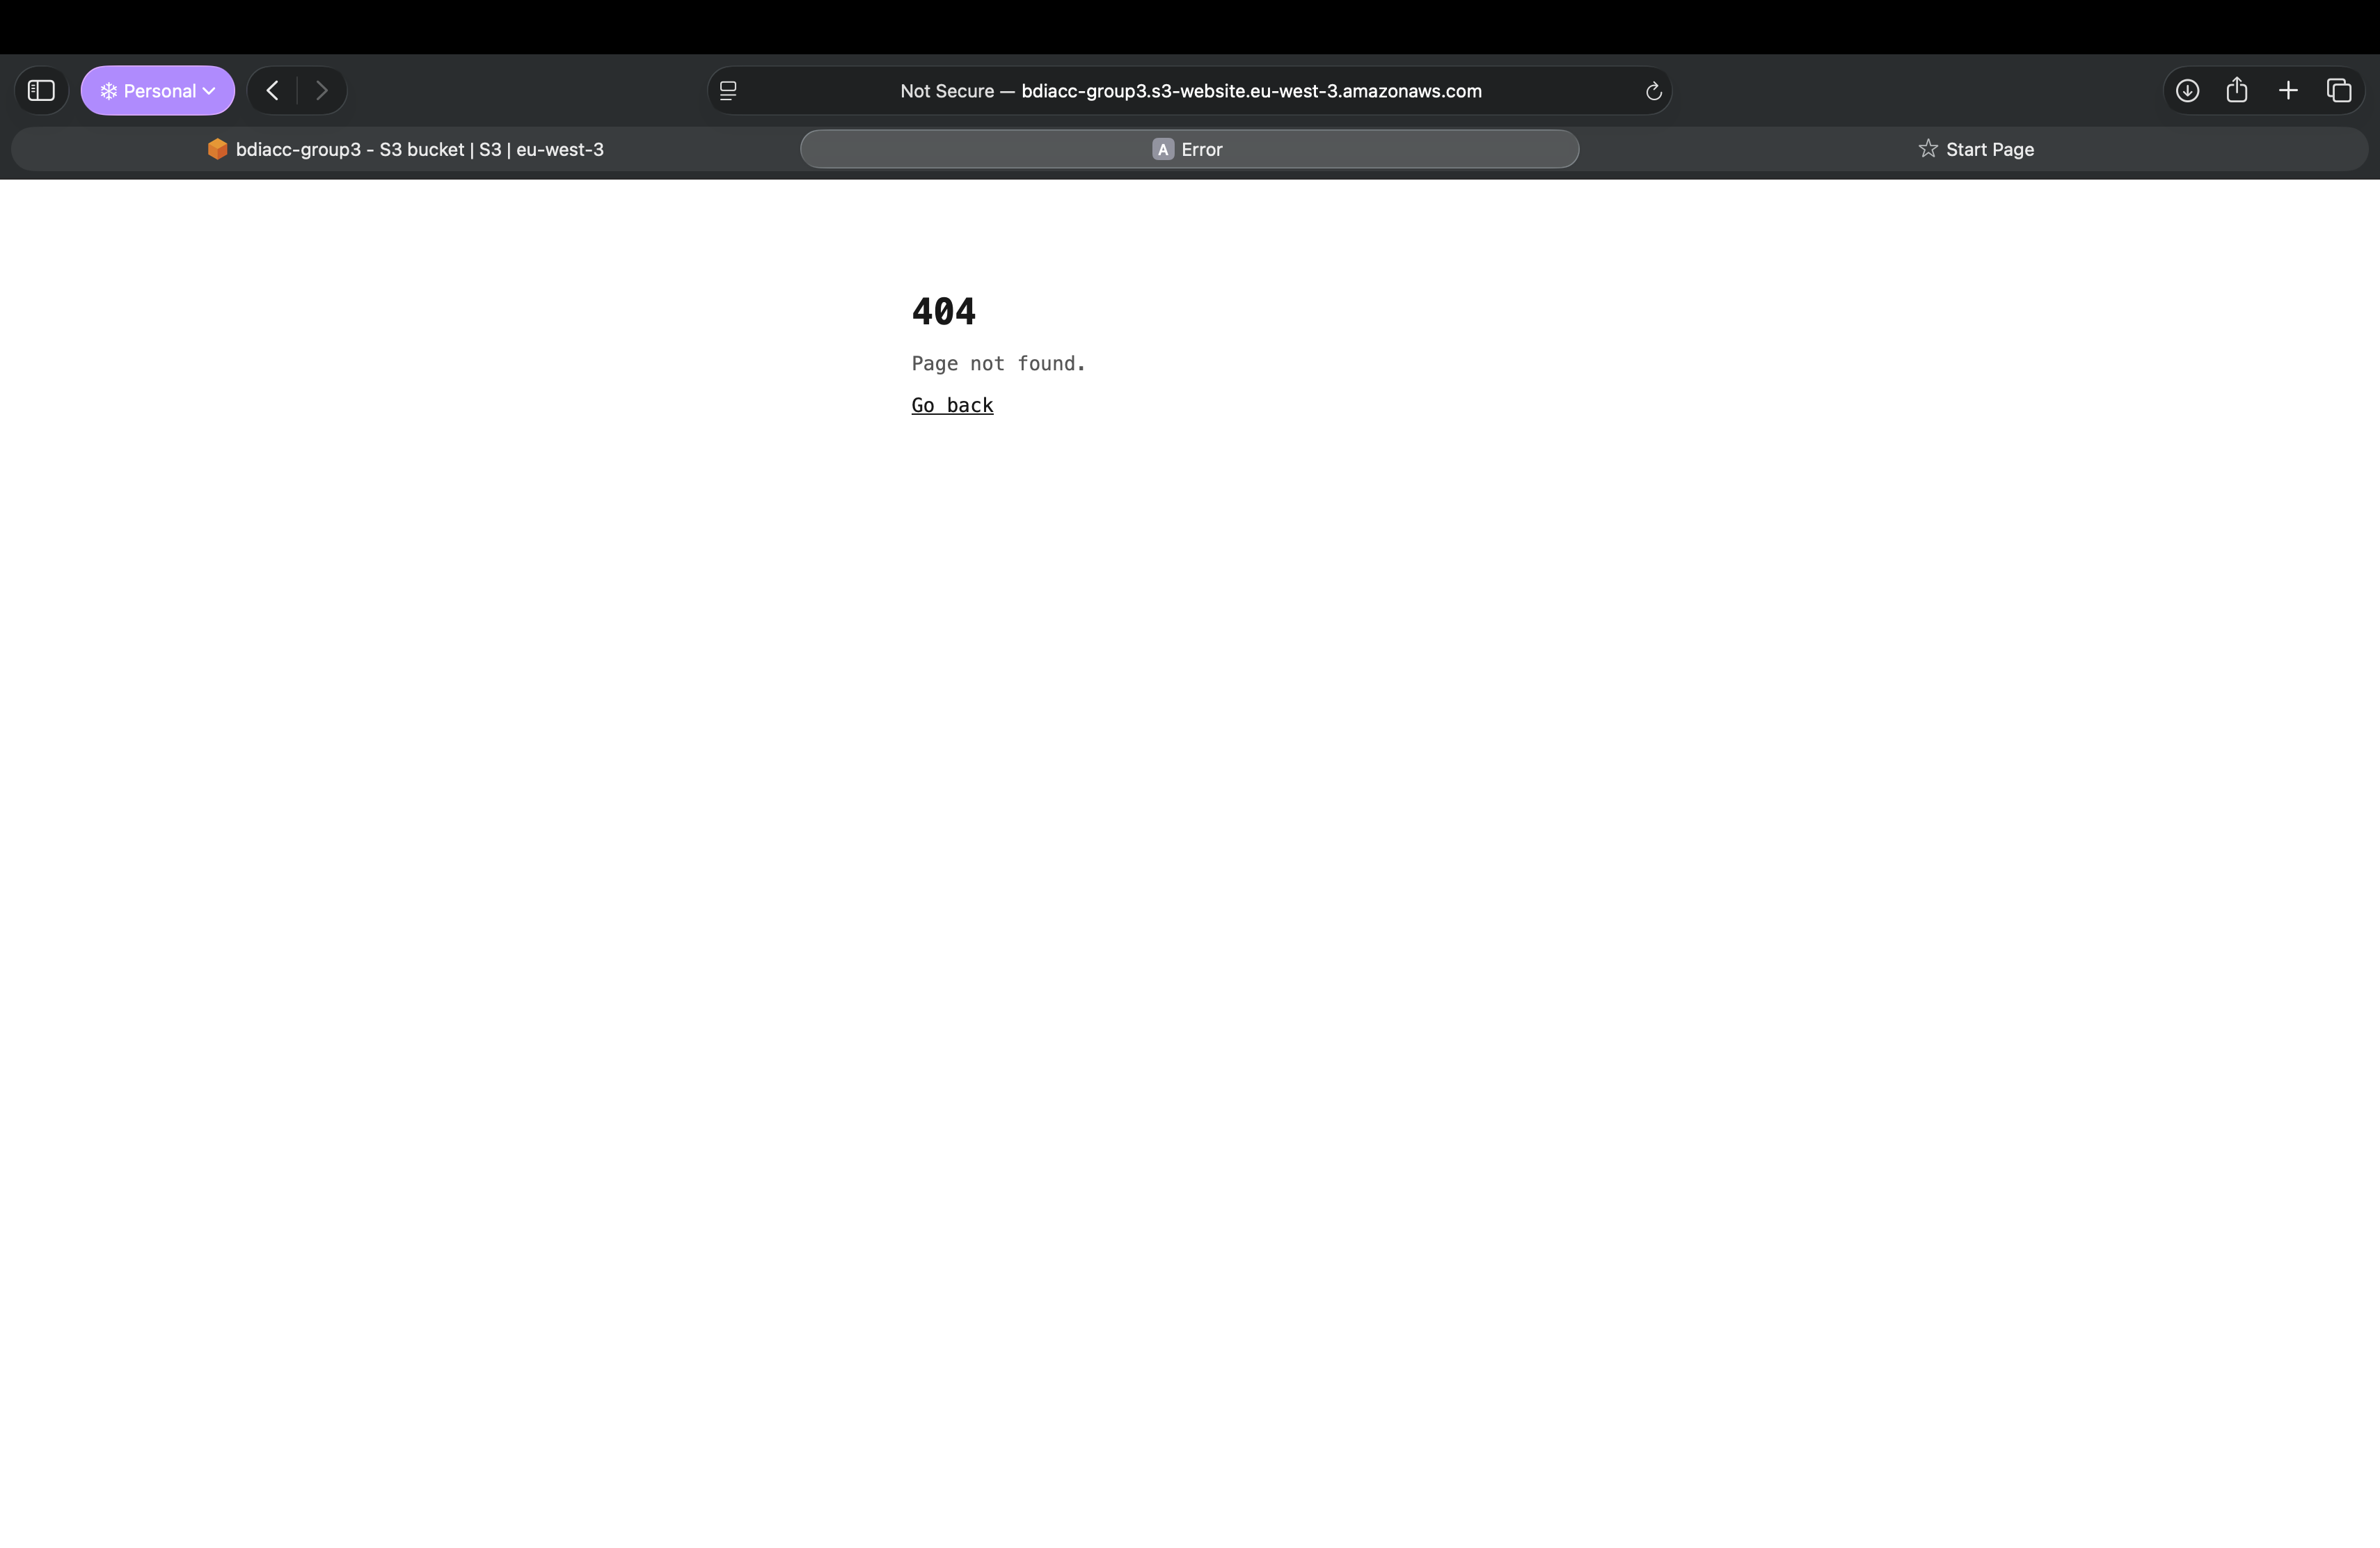
\includegraphics[width=0.75\textwidth]{figures/lab_4/error_html.png}
\caption{Original error.html}
\end{figure}

\textbf{Updated versions:}

When we re-uploaded the files, they got new version IDs:

\begin{itemize}
    \item index.html: \texttt{Xo5opup2H\_I9L5eHRetu\_WswrJkVmNto}
    \item error.html: \texttt{.OZCYhTJt8YmBbY2G3ANgHptOzaMKrDV}
\end{itemize}

\begin{figure}[H]
\centering
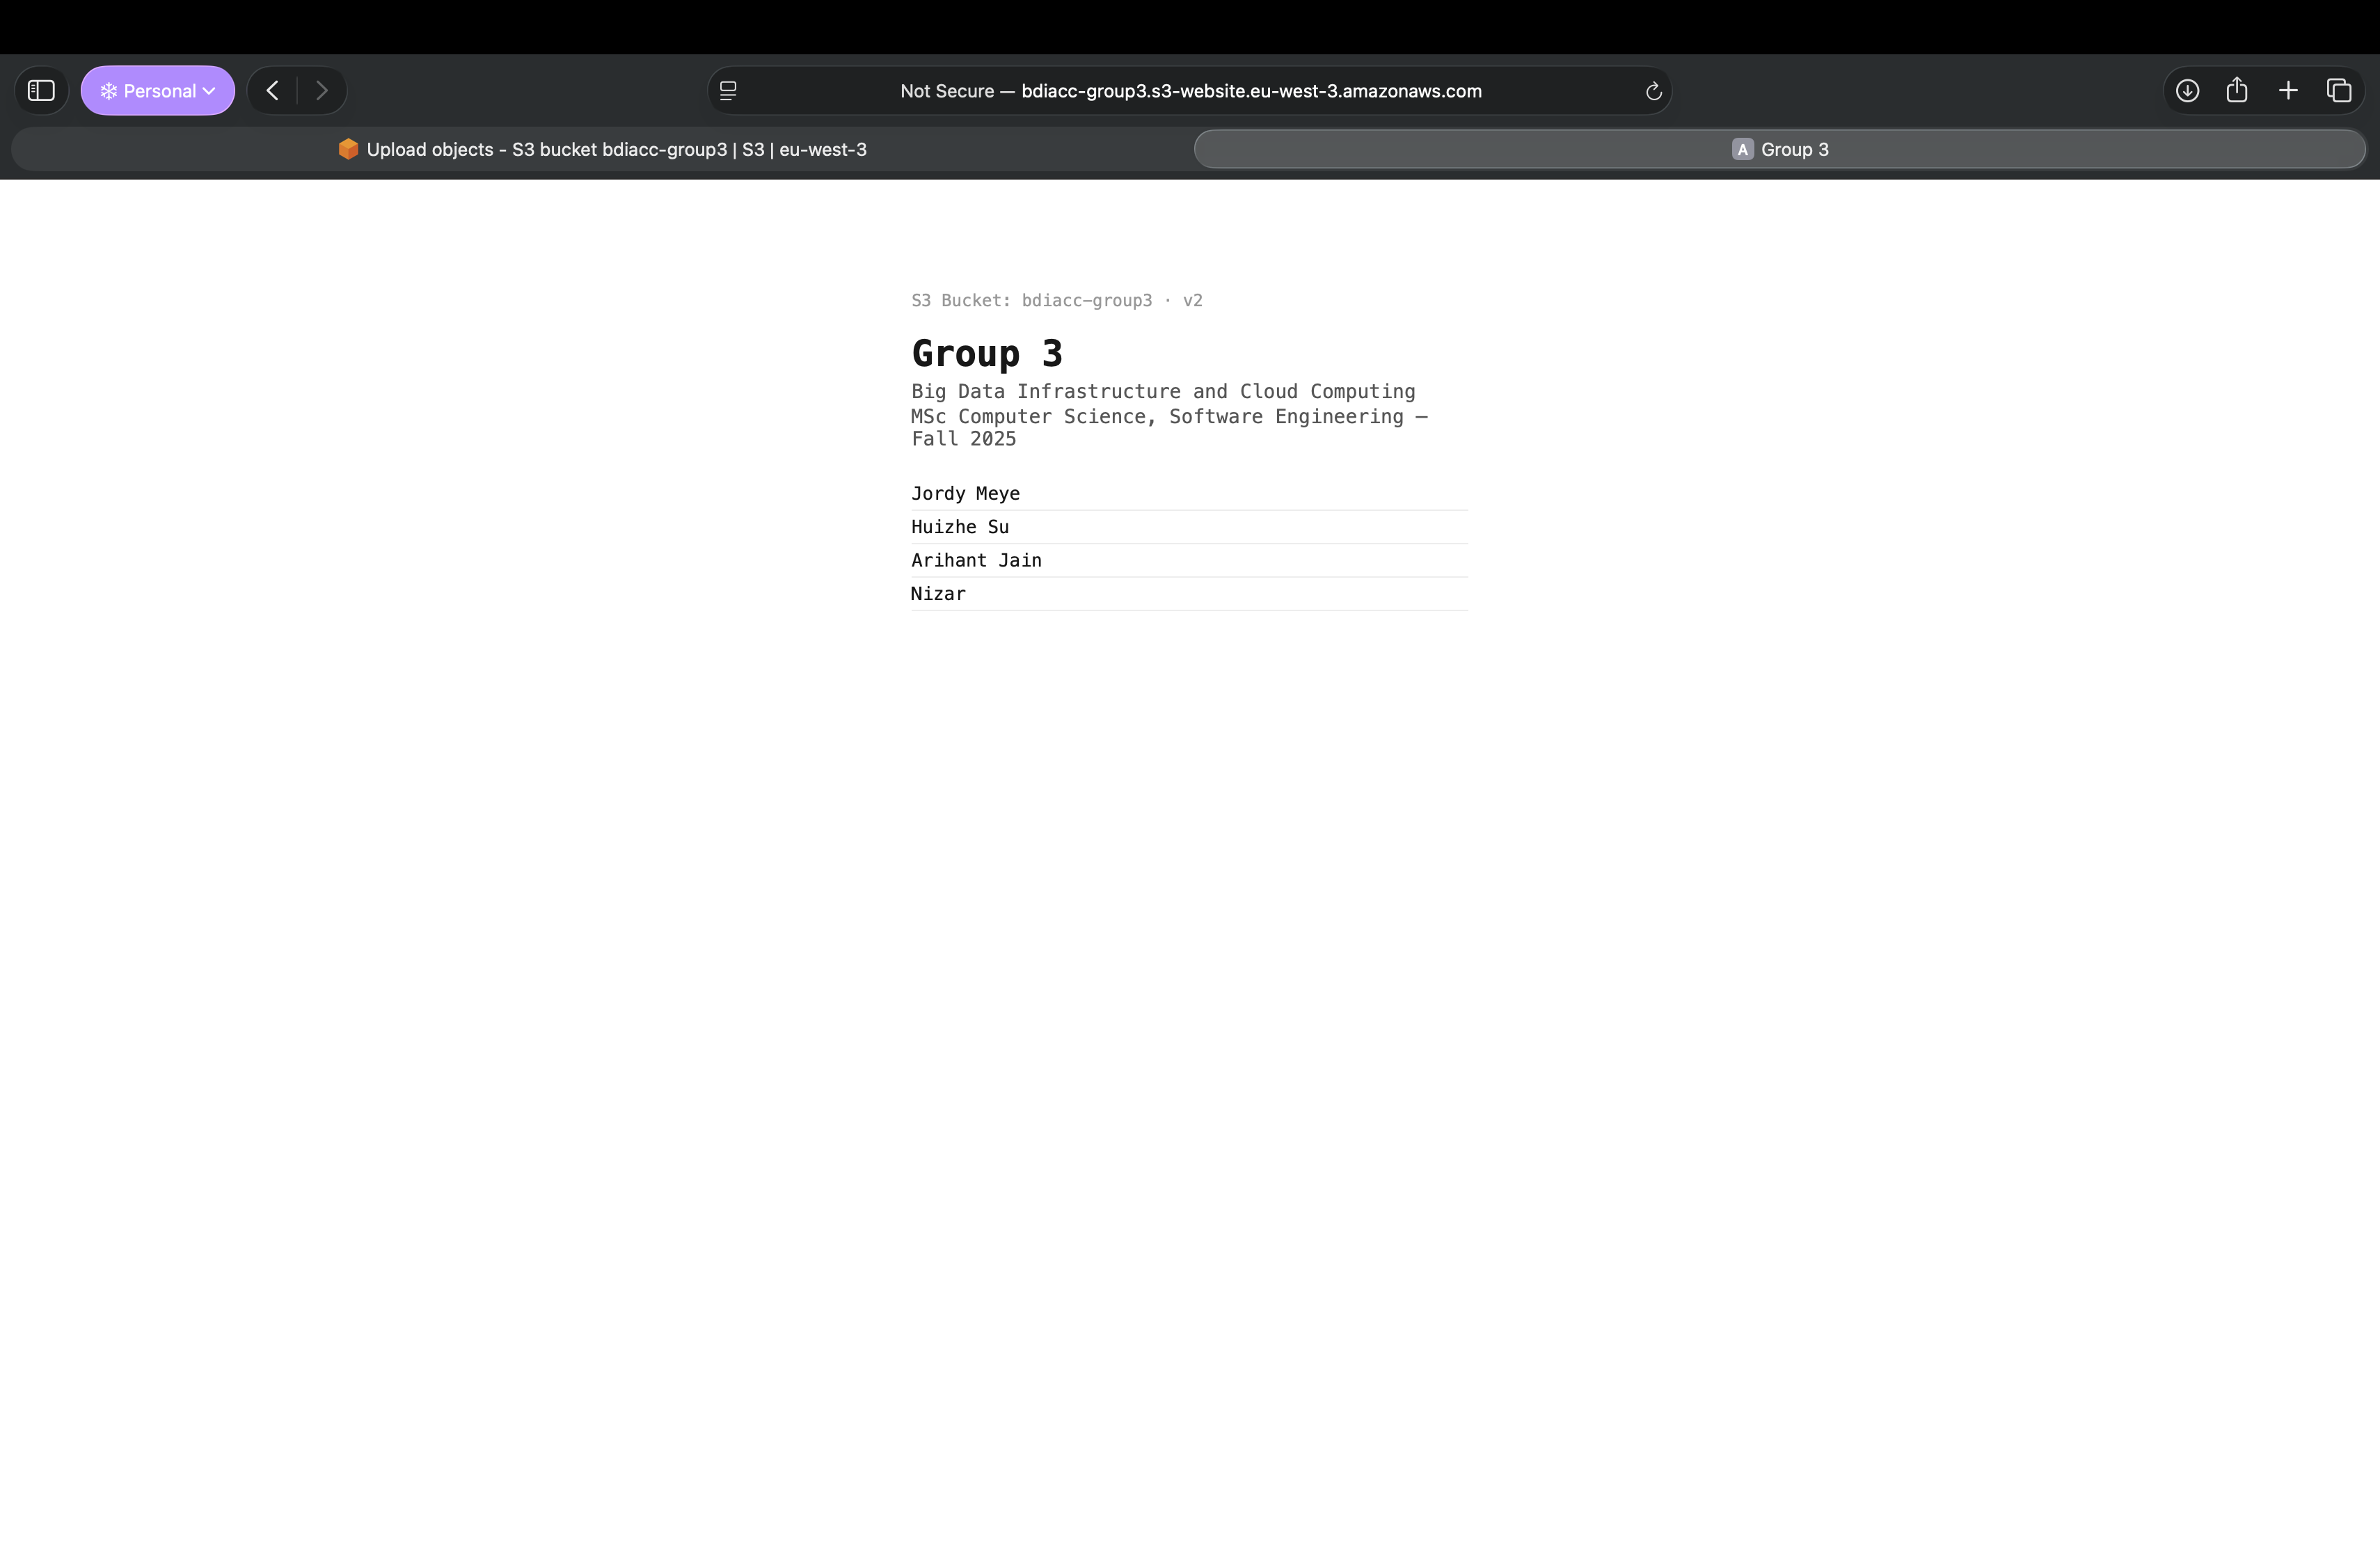
\includegraphics[width=0.75\textwidth]{figures/lab_4/index_html_v2.png}
\caption{Updated index.html}
\end{figure}

\begin{figure}[H]
\centering
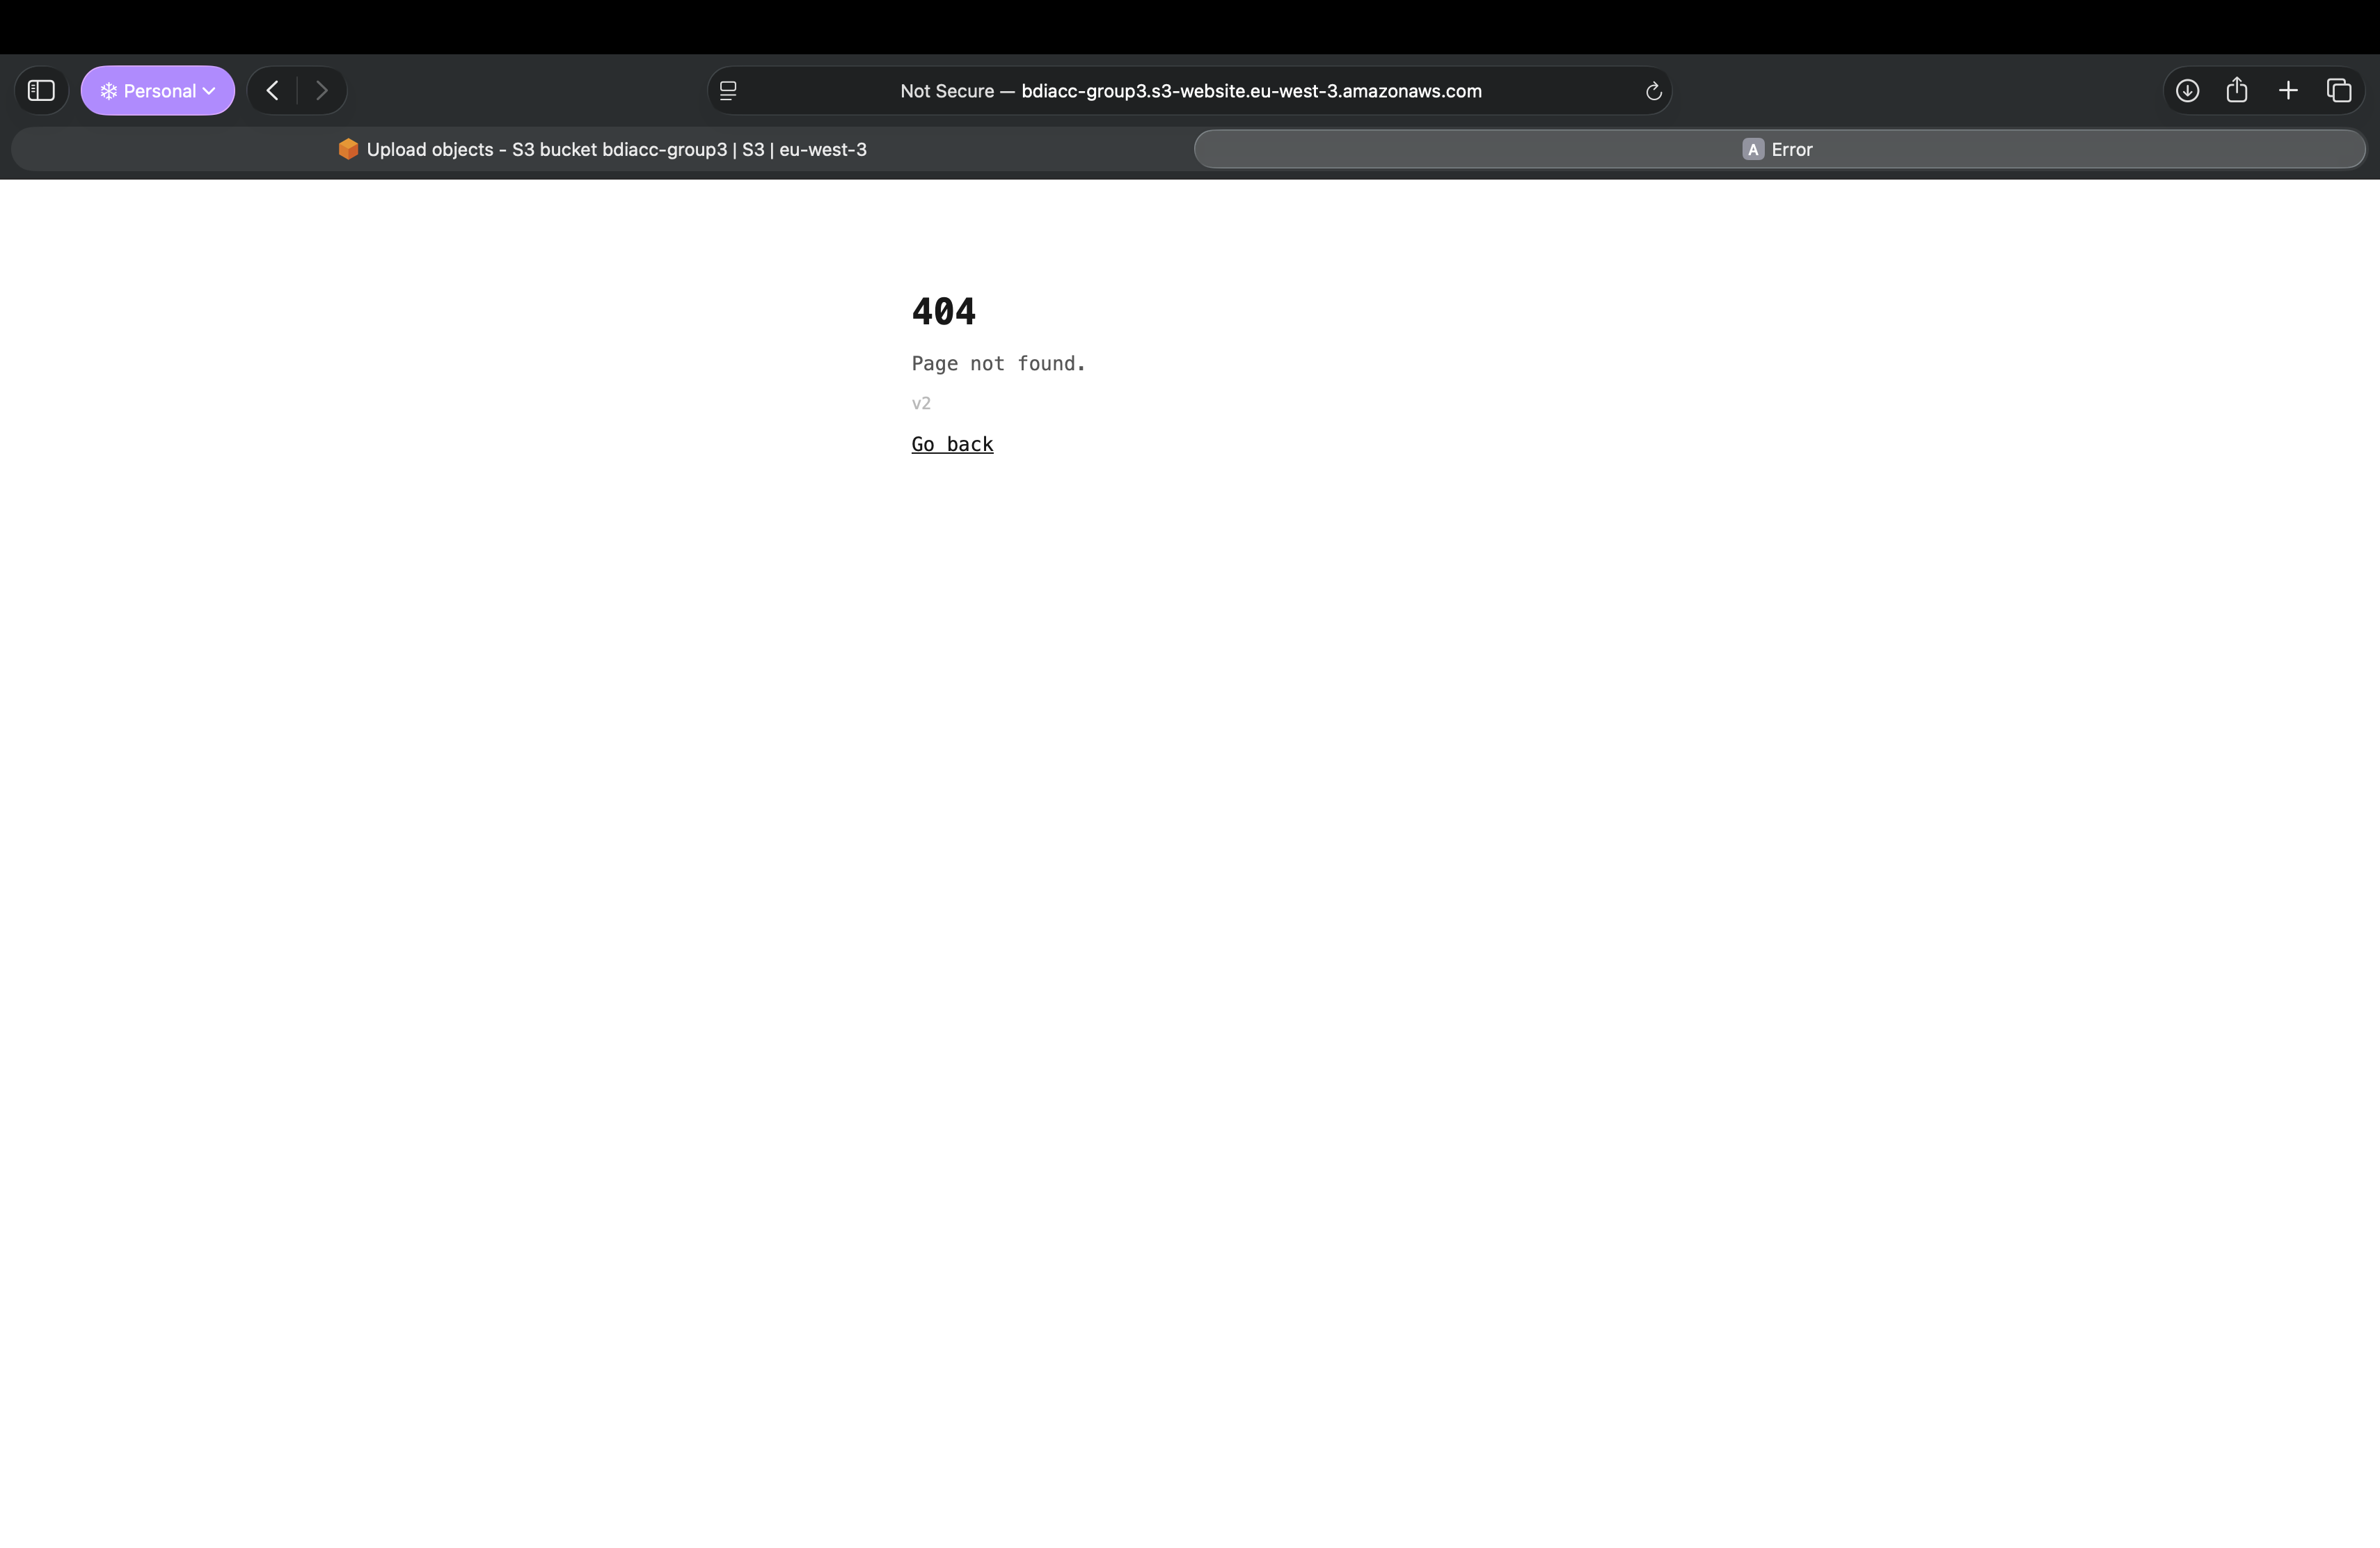
\includegraphics[width=0.75\textwidth]{figures/lab_4/error_html_v2.png}
\caption{Updated error.html}
\end{figure}

\subsection{Verify Multiple Versions in Bucket}

The bucket now contains multiple versions of each file. In the S3 console, both old and new versions are visible.

\begin{figure}[H]
\centering
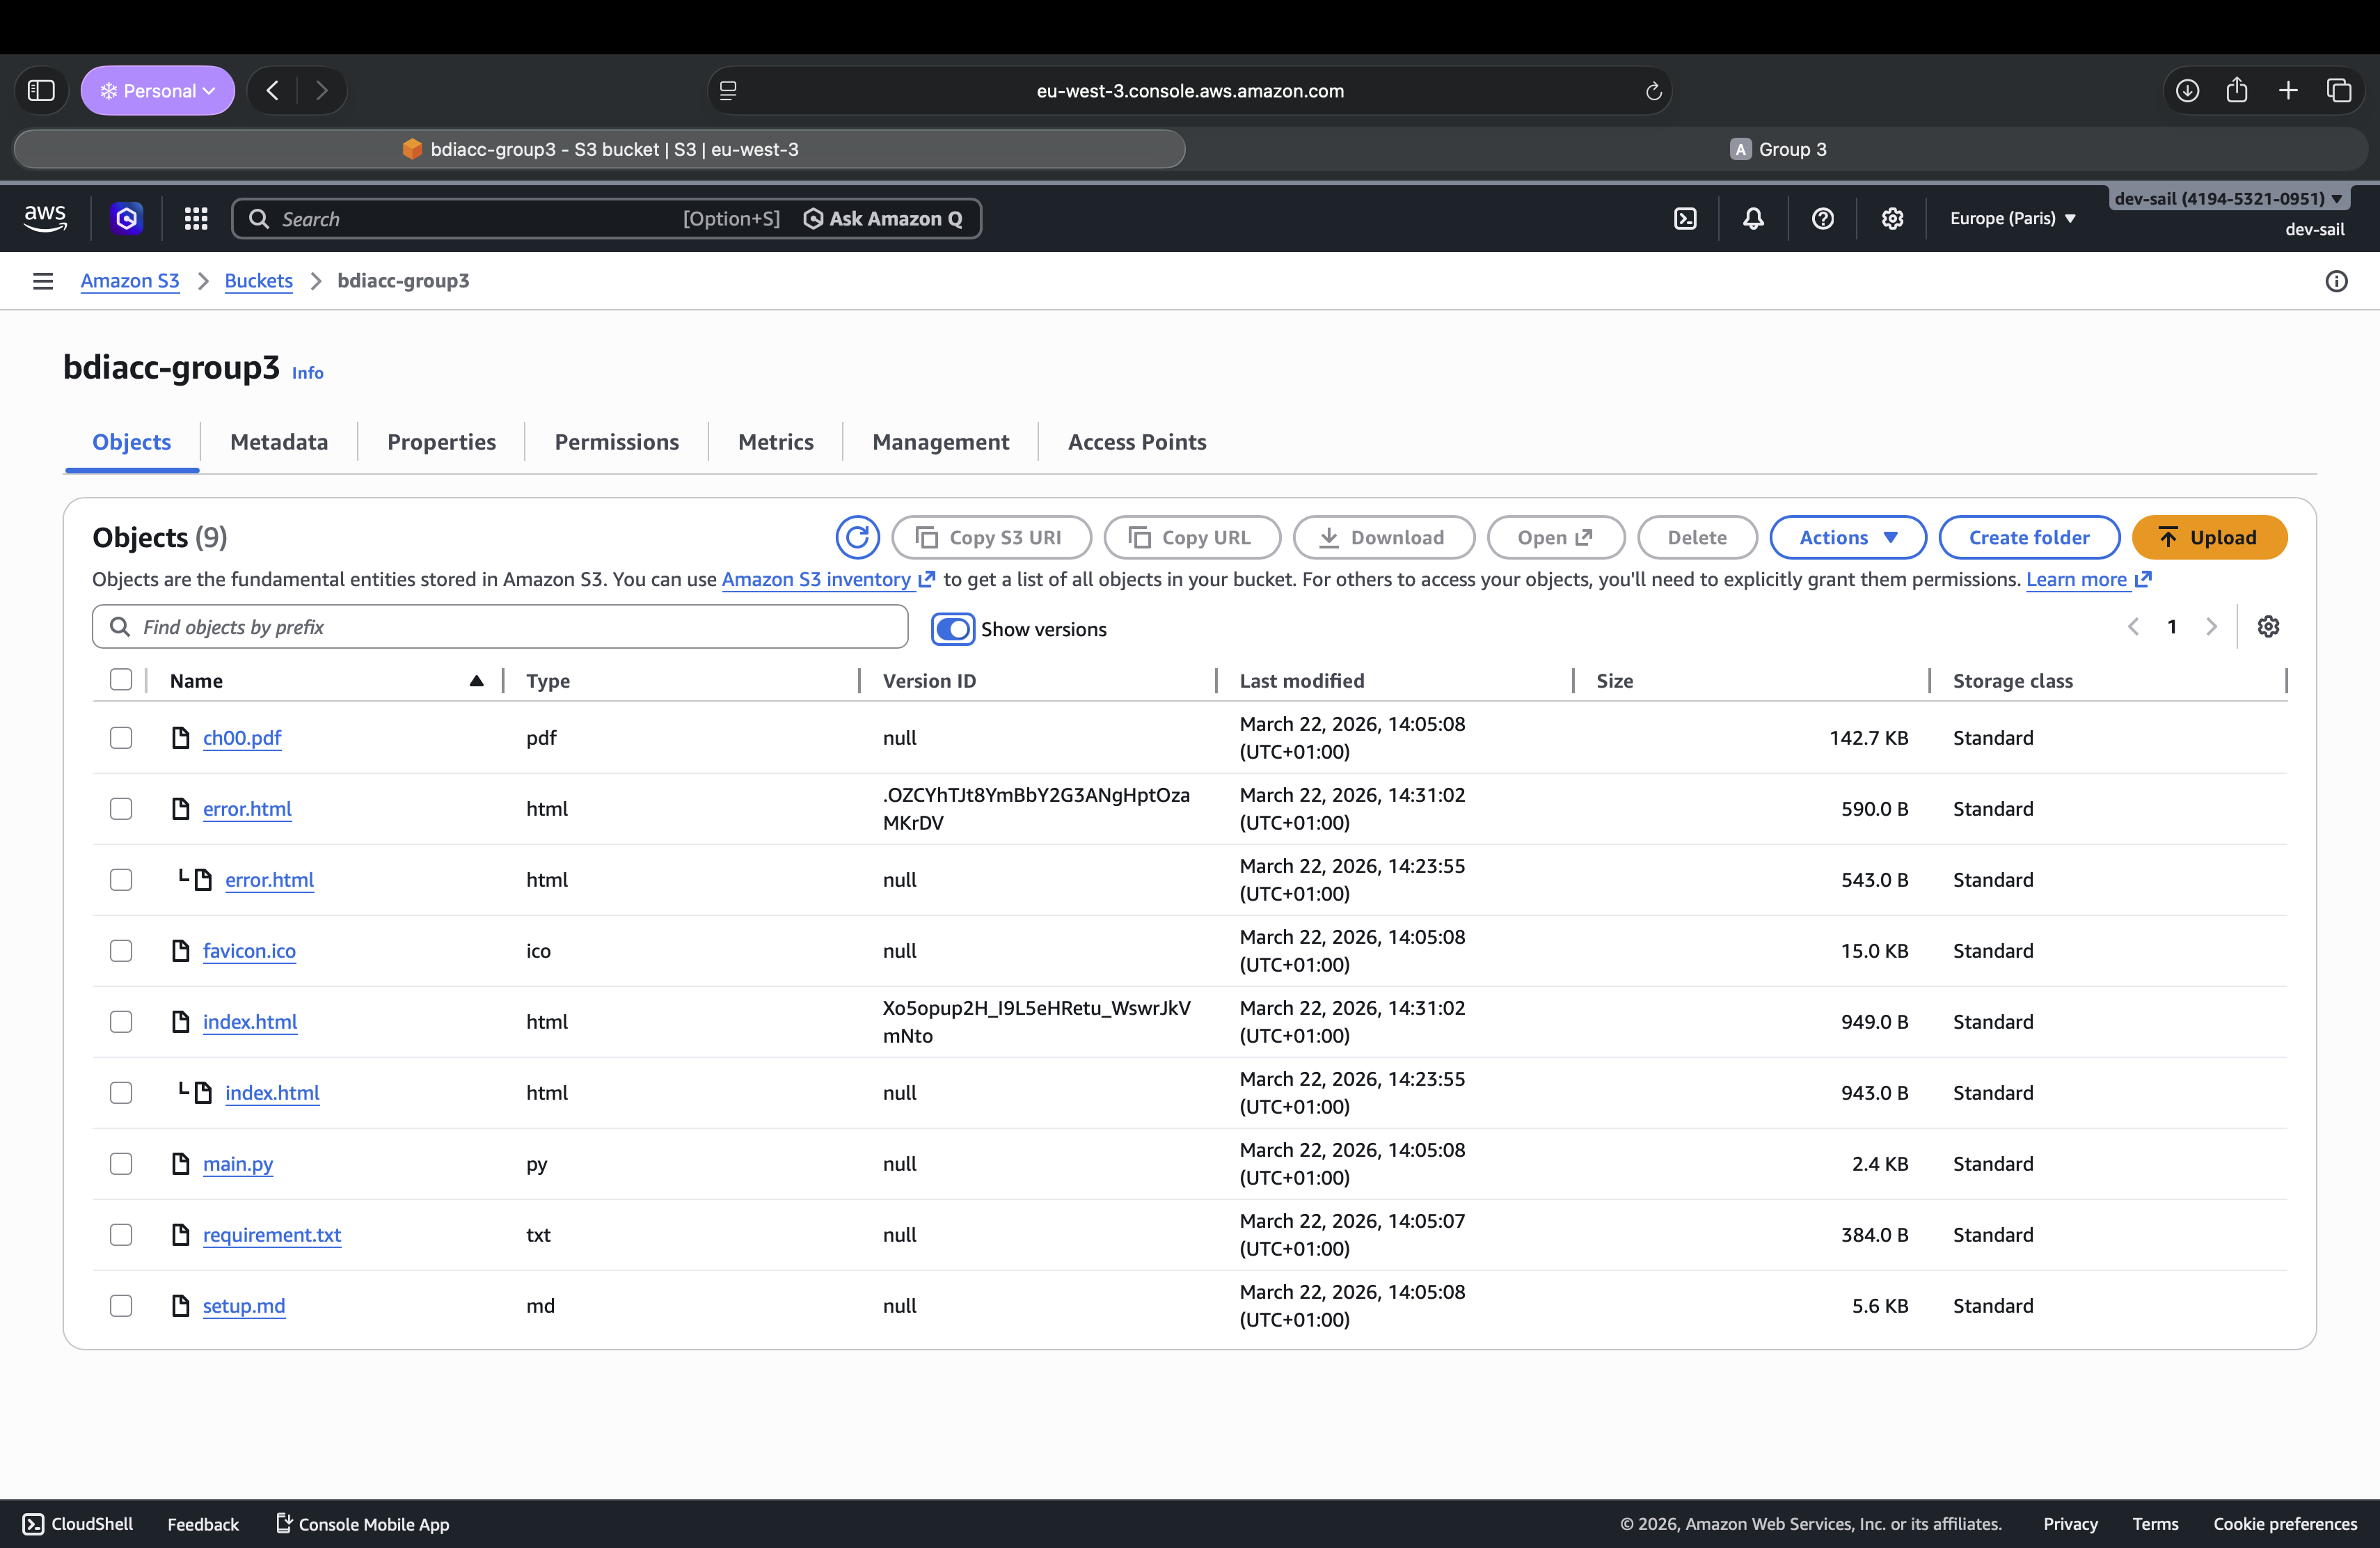
\includegraphics[width=0.75\textwidth]{figures/lab_4/s3_bucket_with_v2_files.png}
\caption{Bucket with multiple file versions}
\end{figure}

The bucket contains:

\begin{itemize}
    \item 9 objects total
    \item index.html: Version ID \texttt{Xo5opup2H\_I9L5eHRetu\_WswrJkVmNto} (949.0 B, 14:31:02) and older version (943.0 B, 14:23:55)
    \item error.html: Version ID \texttt{.OZCYhTJt8YmBbY2G3ANgHptOzaMKrDV} (590.0 B, 14:31:02) and older version (543.0 B, 14:23:55)
    \item Other files: ch00.pdf, favicon.ico, main.py, requirement.txt, setup.md
\end{itemize}

Versioning allows us to restore older versions if a new upload causes problems.

\end{document}
